\documentclass[a4paper, oneside, 12pt]{article}
% 国赛要求，页面布局上下左右都要留出至少 2.5cm
\usepackage[margin=2.5cm]{geometry}

% 编译检查，必须使用 XeLaTeX 编译
\usepackage{iftex}
\ifXeTeX
    \typeout{=> Compiler Check: XeLaTeX detected. Proceeding.}
\else
    \errmessage{COMPILER ERROR: This document MUST be compiled with XeLaTeX.}
\fi

% 中文支持
\usepackage[fontset=none]{ctex}
\usepackage{xeCJK}
\setcounter{secnumdepth}{5} % 为 \subsubsection 增加编号

% 字体设置
\usepackage{anyfontsize}
\usepackage{fontspec}
\setmainfont{Times New Roman} % 英文使用 Times New Roman
\setmonofont{JetBrains Mono}
\setCJKmonofont{KaiTi}

% 使用基础宋体
\setCJKmainfont{SimSun}[
    % BoldFont = SimHei, % 中文粗体使用黑体
    BoldFont = {思源宋体 CN SemiBold},
    ItalicFont = KaiTi, % 中文斜体使用楷体
    BoldItalicFont = KaiTi
]

% 该定义用于附录仿宋字体
\newCJKfontfamily{\fangsong}{FangSong}

% 章节标题
\usepackage{titlesec}
\renewcommand{\thesection}{\chinese{section}}
\titleformat{\section}
{\Large\bfseries\centering}
{\thesection、}
{0em}
{}

\renewcommand{\thesubsection}{\arabic{section}.\arabic{subsection}}
\titleformat{\subsection}
{\large\bfseries}
{\thesubsection}
{1em}
{}

\renewcommand{\thesubsubsection}{\thesubsection.\arabic{subsubsection}}
\titleformat{\subsubsection}
{\normalsize\bfseries}
{\thesubsubsection}
{1em}
{}

% 标题间距调整
\titlespacing{\section}{0pt}{0.2\baselineskip}{0.2\baselineskip}
\titlespacing{\subsection}{0pt}{0.2\baselineskip}{0.2\baselineskip}
\titlespacing{\subsubsection}{0pt}{0.2\baselineskip}{0.2\baselineskip}

% Drawing 绘图板块包
\usepackage{pgfplots}
\usepackage{tikz}
\usepackage{tikz-cd}
\usepackage{tikz-qtree}
\usepackage{circuitikz}
\usepackage{tikz-3dplot}
\usepackage[svgnames]{xcolor}
\pgfplotsset{compat=1.18}
\usetikzlibrary{shapes.geometric, arrows.meta, positioning, calc, angles, quotes, intersections, tikzmark, backgrounds, shadows, fit}

% 代码块设置
\usepackage{mdframed}
\usepackage{fancyvrb}
\usepackage{listings}
\usepackage{algorithm,algorithmic}

\definecolor{lstcolorComment}{rgb}{0,0.6,0}
\definecolor{lstcolorNumber}{HTML}{E6E6E6}
\definecolor{lstcolorString}{rgb}{1,0.5,0}

\lstset{
    backgroundcolor=\color{white},           % 背景色
    basicstyle=\footnotesize\ttfamily,       % 等宽字体和大小
    breakatwhitespace=false,                 % 是否只在空白处断行
    breaklines=true,                         % 自动断行
    keepspaces=true,                         % 保留代码中的空格，对齐代码
    tabsize=2,                               % Tab 长度为 2 个空格
    frame=single,                            % 单线边框
    rulecolor=\color{black},                 % 边框颜色
    captionpos=bl,                           % 标题位置 (bottom-left)
    numbers=left,                            % 行号在左侧
    numbersep=5pt,                           % 行号与代码的距离
    numberstyle=\tiny\color{lstcolorNumber}, % 行号样式
    stepnumber=1,                            % 行号步长
    commentstyle=\color{lstcolorComment},    % 注释样式
    keywordstyle=\color{blue},               % 关键字样式
    stringstyle=\color{lstcolorString},      % 字符串样式
    showspaces=false,                        % 不显示空格
    showstringspaces=false,                  % 不显示字符串中的空格
    showtabs=false,                          % 不显示 Tab
    escapeinside={\%*}{*},                   % 允许在代码中插入 LaTeX 命令
    extendedchars=true                       % 支持非 ASCII 字符 (对旧编码有效)
}

% Matlab 代码块
\usepackage{matlab-prettifier}
\lstdefinestyle{matlab}{
    style=Matlab-Pyglike,         % 基础样式，提供精确的 MATLAB 关键字高亮
    mlshowsectionrules=true,      % 特色功能：高亮 %% 分节符
    backgroundcolor=\color{white},
    basicstyle=\footnotesize\ttfamily,
    numberstyle=\scriptsize\color{mygray}, % 统一使用 mygray 颜色
    frame=single,
    rulecolor=\color{black},
    captionpos=bl,
    breaklines=true,
    keepspaces=true,
    numbers=left,
    numbersep=8pt,
    showstringspaces=false,
    tabsize=2,
    keywordstyle=\color{deepblue}\bfseries, % 关键字：深蓝、粗体
    commentstyle=\itshape\color{black!35!white}, % 注释：斜体、浅灰
    stringstyle=\color{orange},          % 字符串：橙色
    identifierstyle=\color{myidentifier},  % 标识符(变量/函数名)：深青色
}

% Python 代码块
\usepackage{color}
\definecolor{mygray}{rgb}{0.5,0.5,0.5}
\definecolor{brightgreen}{RGB}{0, 135, 0}
\definecolor{deepblue}{rgb}{0,0,0.5}
\definecolor{deepred}{rgb}{0.6,0,0}
\definecolor{lightblue}{RGB}{91, 192, 255}
\definecolor{orange}{rgb}{1,0.5,0}
\definecolor{myidentifier}{rgb}{0.2,0.4,0.6} % 为标识符高亮深青色
\lstdefinestyle{python}{
    language=Python,
    backgroundcolor=\color{white},          % 背景色
    basicstyle=\footnotesize\ttfamily,      % 代码字体：小号、等宽
    numberstyle=\scriptsize\color{mygray},  % 行号字体：更小号、灰色
    identifierstyle=\color{myidentifier},   % 标识符字体：深蓝
    frame=single,                           % 单线边框
    rulecolor=\color{lightblue},               % 边框颜色
    captionpos=bl,                           % 标题位置：左下角
    keywordstyle=\color{orange}\bfseries, % 关键字：深蓝、粗体
    commentstyle=\itshape\color{black!35!white}, % 设置注释样式，斜体，浅灰
    stringstyle=\color{brightgreen},             % 字符串：橙色
    morekeywords={self},                    % 额外关键字
    emph={MyClass,__init__, GCN, GAT, self},      % 强调词列表
    emphstyle=\color{deepred}\bfseries,     % 强调词样式：深红、粗体
    breaklines=true,                        % 自动断行
    keepspaces=true,                        % 保留空格，用于对齐
    numbers=left,                           % 行号在左
    numbersep=8pt,                          % 行号与代码间距
    showstringspaces=false,                 % 不显示字符串中的空格
    tabsize=2                               % Tab 长度
}

% Darcula Theme
\definecolor{Darcula-bg}{RGB}{43, 43, 43}        % 背景色 (深灰)
\definecolor{Darcula-fg}{RGB}{169, 183, 198}      % 前景色/普通文本 (亮灰)
\definecolor{Darcula-comment}{RGB}{128, 128, 128}   % 注释 (灰色)
\definecolor{Darcula-keyword}{RGB}{204, 120, 50}    % 关键字 (橙色)
\definecolor{Darcula-function}{RGB}{255, 203, 107}  % 函数名 (黄色)
\definecolor{Darcula-string}{RGB}{106, 135, 89}     % 字符串 (绿色)
\definecolor{Darcula-variable}{RGB}{152, 118, 170} % 变量与参数 (淡紫色)
\definecolor{Darcula-number}{RGB}{104, 151, 187}   % 数字 (蓝色)

\lstdefinestyle{darcula}{
    language=Python,
    backgroundcolor=\color{white},
    basicstyle=\small\ttfamily\color{Darcula-fg},
    frame=single,
    rulecolor=\color{Darcula-keyword},
    captionpos=b,
    keywordstyle=\color{Darcula-keyword},
    stringstyle=\color{Darcula-string},
    commentstyle=\itshape\color{Darcula-comment},
    numberstyle=\tiny\color{Darcula-number}, % 行号也用数字的蓝色
    identifierstyle=\color{Darcula-variable},
    emph={read_csv, merge, rename},
    emphstyle=\color{Darcula-function},
    morekeywords=[2]{True, False, None},
    keywordstyle=[2]\color{Darcula-keyword},
    breaklines=true,
    keepspaces=true,
    numbers=left,
    numbersep=10pt,
    showstringspaces=false,
    tabsize=4,
}

% TColorbox
\usepackage[many]{tcolorbox}
\usepackage{fontawesome5}

\definecolor{warningRed}{RGB}{217, 83, 79}
\definecolor{warningRedBack}{RGB}{242, 222, 222}

\newtcolorbox{warning}{
    enhanced,
    shadow={0.8mm}{-0.8mm}{0mm}{black!20!white},
    breakable, % 允许内容跨页
    colback=warningRedBack, % 背景颜色
    colframe=warningRed,    % 边框颜色
    boxrule=0.5pt,          % 边框线宽
    leftrule=2pt,           % 左侧竖线的宽度 (比边框粗，更明显)
    top=2pt,
    bottom=1.8pt,
    right=5em,
    fontupper=\fontsize{9.5pt}{13pt}\selectfont\kaishu,
    fonttitle=\small\bfseries,
    title={
            \faExclamationTriangle[solid]
            \hspace{1.5pt}
            \textbf{Warning}
        },
    coltitle=white,
    attach boxed title to top right={xshift=0pt, yshift=-18.3pt},
    boxed title style={
            colback=warningRed,
            boxrule=0.3pt,
        }
}

\definecolor{tipBlue}{RGB}{91, 192, 222}
\definecolor{tipBlueBack}{RGB}{217, 237, 247}

\newfontfamily{\kaishu}{KaiTi}
\newtcolorbox{tips}{
    enhanced,
    shadow={0.8mm}{-0.8mm}{0mm}{black!20!white},
    breakable,
    colback=tipBlueBack,    % 背景颜色
    colframe=tipBlue,       % 边框颜色
    boxrule=0.5pt,          % 边框线宽
    leftrule=2pt,           % 左侧竖线的宽度
    top=2pt,
    bottom=1.8pt,
    right=5em,
    fontupper=\fontsize{9.5pt}{13pt}\selectfont\kaishu, % 内容字体: {大小}{衬线}
    fonttitle=\small\bfseries,
    title={
            \faLightbulb[solid]
            \hspace{1.5pt}
            \textbf{Tips}
        },
    coltitle=white,
    attach boxed title to top right={xshift=0pt, yshift=-18.3pt},
    % attach boxed title to top left={xshift=10pt, yshift=-10pt},
    boxed title style={
            colback=tipBlue,
            boxrule=0.3pt,
        }
}

% 行距、缩进
\usepackage{setspace}
\usepackage{indentfirst,comment}
\renewcommand{\baselinestretch}{1.3}
\setlength\parindent{2\ccwd} % 中文两字符缩进

% 颜色支持
\usepackage[table]{xcolor}
\definecolor{structurecolor}{RGB}{60,113,183}
\definecolor{main}{RGB}{0,166,82}
\definecolor{second}{RGB}{255,134,24}
\definecolor{third}{RGB}{0,174,247}
\definecolor{winered}{rgb}{0.5,0,0}
\definecolor{bule}{RGB}{18,29,57}
\colorlet{coverlinecolor}{second}

% Math:
\usepackage{array}
\usepackage{sansmath}
\usepackage{amsmath,mathrsfs,amsfonts,amssymb}
\usepackage{esint}
\usepackage{cases}
\usepackage{bm} % 粗体数学符号
\let\Bbbk\relax % 兼容性处理

% 特殊符号
\usepackage{pifont,manfnt,bbding}
\usepackage{adforn}
\usepackage{csquotes} % 引号

% 脚注
\usepackage[flushmargin,stable]{footmisc}
\setlength{\footnotesep}{12pt}

% 图表
\usepackage{tabularx}
\usepackage{booktabs}
\usepackage{multicol,multirow}
\usepackage{makecell}
\usepackage{graphicx}
\usepackage{siunitx}    % 提供 S 列类型，用于对齐数字
\usepackage[hypcap=false, labelfont={bf,color=structurecolor}]{caption}
\usepackage{float}
\usepackage{subcaption}
\captionsetup[table]{skip=0.6\baselineskip, aboveskip=0.6\baselineskip}
\captionsetup[figure]{skip=0.6\baselineskip, aboveskip=0.6\baselineskip}
\captionsetup{
    font=bf,
    labelfont=bf,
    labelsep=quad,
    justification=centering,
    singlelinecheck=true,
    skip=1em
}
\newcommand\figref[1]{\textbf{图}~\ref{#1}}
\newcommand\tabref[1]{\textbf{表}~\ref{#1}}

% 列表，设置了 Itemize 和 Enumerate 不缩进
\usepackage{enumitem}

\setlist[itemize]{
    parsep=\parskip,
    topsep=6pt,
    itemsep=1pt,
    leftmargin=*
}

\setlist[enumerate,1]{
    parsep=\parskip,
    topsep=6pt,
    label=\arabic*., % 标签格式为 1., 2., ...
    leftmargin=* % 标签对齐
}

\setlist[enumerate,2]{
    label=(\alph*),  % 标签格式为 (a), (b), ...
    leftmargin=*,
    topsep=1pt,
    itemsep=0pt
}

% 参考文献
\usepackage[
    backend=biber,          % 指定后端为 biber
    style=gb7714-2015,      % 使用国标 GBT7714-2015 样式
    citestyle=numeric-comp  % 引用为数字压缩格式，如 [1-3]
]{biblatex}
\addbibresource[location=local]{references.bib} % 指定你的 .bib 文件

% \usepackage[numbers,sort&compress]{gbt7714} % 存在多篇引文时自动压缩引号
% \bibliographystyle{gbt7714-numerical}
% \setcitestyle{super=false}
% \renewcommand{\citenumfont}[1]{\textbf{#1}}

% 附录
\usepackage[header]{appendix}
\usepackage{titlesec}

% 只在第一次调用 \addappendix 时执行
\newcommand{\addappendix}[1]{
    \appendix

    \titleformat{\section}
    {\large\bfseries\centering}
    {附录~\thesection}
    {1em}
    {}

    \titlespacing*{\section}{0pt}{2em}{1em}

    % 将 \addappendix 命令重定义为一个简单的 \section 命令
    % 后续再调用 \addappendix 时，就不会重复执行上面的设置了
    % 这里用 ##1 是因为在 \newcommand 的定义中)
    \renewcommand{\addappendix}[1]{\section{##1}}
    \refstepcounter{section}
    \section*{附录~\thesection\hspace{1em}#1}
}
% 此处让 \addappendix 命令暂时处于不进入目录的状态

% 超链接
\usepackage{hyperref}
\hypersetup{
    breaklinks,
    unicode,
    linktoc=all,
    bookmarksnumbered=true,
    bookmarksopen=true,
    colorlinks=true,
    linkcolor=black,
    citecolor=black,
    urlcolor=blue,
    plainpages=false,
    pdfstartview=FitH,
    pdfborder={0 0 0},
    linktocpage
}

\newcommand{\h}{\hspace}
\renewcommand{\v}{\vspace}

\AtBeginDocument{
    \setlength{\abovedisplayskip}{0.45em}
    \setlength{\belowdisplayskip}{0.6em}
}
\usepackage{ragged2e}
\usepackage{tabularx}

\begin{document}

\section*{基于混合模型的 NIPT 检测时点选择与胎儿异常判定}

\v{0.2em}

\begin{center}
    \large\bfseries
    摘要
\end{center}

\v{-0.5em}

\textbf{针对问题一}，本文首先通过\textbf{方差膨胀因子（VIF）}分析消除了身高、体重的多重共线性，并结合统计检验与文献研究排除了孕妇年龄与生产次数的显著影响。考虑到数据为\textbf{重复测量数据}，其观测值不满足独立性假设，本文计算了\textbf{组内相关系数（ICC）}为 $0.5984$，证明了采用混合效应模型的必要性。最终，通过\textbf{AIC/BIC}准则在多个候选模型中进行择优，建立了一个\textbf{非线性混合效应模型}：$Y = 0.218290 - 0.011993 w + 0.000326 w^2 - 0.002045 \text{BMI} + 0.012028 c$。该模型中所有变量的$p$值均远小于$0.05$，具有高度统计显著性，且模型的\textbf{条件 $R^2$ 值达到 $0.7664$}，表现出强大的解释能力。

\textbf{针对问题二}，为给BMI体型的孕妇提供个性化的NIPT时点建议，本文构建了一个\textbf{带约束的多目标优化模型}。模型旨在\textbf{最小化潜在风险}，同时\textbf{最大化检测成功率}。本文采用 \textbf{K-Means聚类分析} 验证了将孕妇\textbf{分为 $4$ 组}的合理性。随后建立了随孕周递增的\textbf{分段式风险函数}，并通过\textbf{加权和法}将多目标转化为单目标。为确保方案的临床可行性，模型引入了\textbf{两周的检测窗口}，并对窗口施加了\textbf{上下限约束}。最终，使用\textbf{SLSQP求解器}成功捕获了\textbf{四个最优的BMI分组区间}及最佳NIPT检测窗口。通过\textbf{组内对比}分析与精美的\textbf{可视化验证}，证明该方案可在风险与成功率之间做出智能权衡。

\textbf{针对问题三}，本文在\textbf{问题一、二的基础上}，综合考虑\textbf{检测误差}与\textbf{样本达标率}，构建了一个包含\textbf{核心、硬性及逻辑等多重约束的优化模型}。该模型核心要求推荐检测时点的预测Y染色体浓度\textbf{不低于$6\%$}，并利用\textbf{差分进化算法}求解最佳 BMI 分组方案与对应的检测窗口。为不同孕妇提供了最佳 NIPT 时点建议，模型显示：对于\textbf{高BMI孕妇}，模型推荐的较晚孕周窗口能将检测成功率\textbf{提升近$15\%$}；而对于\textbf{中低BMI孕妇}，模型则在保障高成功率的同时，兼顾了早期检测的临床效益。

\textbf{针对问题四}，本文提出了一种基于\textbf{优化XGBoost模型}的女胎染色体异常综合判定方法。为解决数据中异常样本稀疏导致的类别严重不平衡问题，本文采用\textbf{SMOTETomek混合采样技术}对训练集进行预处理，有效生成了少数类样本。随后结合网格搜索与交叉验证进行超参数寻优。考虑到临床诊断中\textbf{“漏诊”的严重性远高于“误诊”}，优化过程以召回率为核心评估指标，旨在最大化对异常胎儿的检出能力。为将模型的\textbf{概率预测转化为科学的二元判定}，本文通过遍历所有可能的决策阈值，找到了使\textbf{F1分数达到最大值的最优决策点}。该最优阈值代表了模型在低误诊与低漏诊之间的最佳平衡。由此，本文确立了最终判定方法：当模型输出的\textbf{异常概率大于最优阈值 0.8128 时，即判定女胎为“异常”}。该方法综合了多维生理指标，并通过科学的阈值选择，为临床辅助诊断提供了可靠、量化的决策依据。

\v{1em}

\noindent
\textbf{关键词}：无创产前检测 \quad 非线性混合效应 \quad 约束优化 \quad XGBoost

\newpage

% \tableofcontents

% \begin{warning}
%     国赛要求提交时必须删除目录，这是写作便于组织结构的！
% \end{warning}

% \newpage

\section{引言}

\subsection{问题背景}

产前检测，即通过孕妇的早期检测来确定胎儿的健康状况的方法，近年来得到了广泛的关注和应用。无创产前检测(NIPT)作为一种简单且低风险的筛查检测，已展现出良好的前景。世界各国政府和私人组织也开始投入大量资源，目的是将其纳入国家医疗保健计划\cite{jayashankar2023non}。

NIPT的具体机制是分析母体血浆中的胎儿游离DNA来进行染色体非整倍体筛查，其核心优势在于准确性高且对孕妇和胎儿无创伤风险。然而，它的性能高度依赖于母体血浆中胎儿游离DNA的占比，即胎儿分数。胎儿分数跟孕妇的体重或身体质量指数（BMI）、孕周数和孕情等都具有可能的相关性，不同孕妇群体的最适检测时间也各不相同。此外，NIPT的准确性并非完美。即便是检测成功，结果也可能与最终的临床诊断不符。

因此如何根据孕妇的个体特征来确定最佳的检测时点，从而平衡检测成功率与时效性，是本文需要解决的核心问题。

\subsection{问题重述}

本文需要在附件中利用的NIPT实际检测数据，建立一系列数学模型，以解决NIPT在临床应用中的时点选择与异常判定问题。同时，注意到问题一至三均聚焦于男性胎儿，问题四则聚焦于女性胎儿。

针对问题一：需要探索并量化男性胎儿Y染色体浓度与孕妇孕周、BMI等关键生理指标之间的数学关系，并对模型的显著性进行检验。

针对问题二：由于孕妇的BMI对男性胎儿的NIPT结果准确性有重要影响，因此需要对孕妇进行合理的BMI分组，并为每组确定一个最佳NIPT检测时点。该时点的选择需要使孕妇因检测时机不当而可能面临的潜在综合风险最小化，同时分析检测误差对结果的影响。

针对问题三：基于问题二的结果，不仅需要对BMI进行考虑，还要综合考虑孕妇的身高、体重、年龄等更多因素，以及检测误差和男性胎儿的 Y 染色体浓度达标比例进行分组。该时点的选择同样需要使得孕妇潜在综合风险最小化，同时分析检测误差对结果的影响。

针对问题四：由于女性胎儿无Y染色体，因此需要利用女胎 21、18、13 号和X染色体的 Z 值、GC 含量、测序读段数及孕妇 BMI 等一系列特征，构建一个高效准确的分类模型，用于判定女性胎儿是否存在染色体非整倍体异常。

\section{问题分析}

\subsection{问题一的分析}

针对问题一，为了避免多重共线性问题对模型稳定性的影响，本文采用方差膨胀因子进行检验。此外，通过数据分析和文献支撑，本文排除了孕妇年龄和生产次数这两个在本次数据集中不具备显著影响的因素。在模型选择阶段，注意到数据集中存在对同一孕妇进行多次检测的特征，属于重复测量数据，因此本文决定采用非线性混合效应模型。对于模型构建与显著性检验，本文设定了多个包含孕周、BMI以及检测次数的非线性候选模型，并利用赤池信息准则（AIC）和贝叶斯信息准则（BIC）进行择优。择优完成后对最优模型进行拟合，而后通过沃尔德检验验证变量的系数的统计显著性。

\subsection{问题二的分析}
针对问题二，目标是构建一个能平衡临床风险与检测成功率的优化决策模型。采用K-Means聚类，根据数据自身特性将孕妇客观地划分为4个BMI组，为后续优化提供分组基础。而后建立多目标优化模型，其核心是“最小化潜在风险”与“最大化检测成功率”之间寻求最佳平衡。通过加权和法将此多目标问题转化为单目标，并以BMI分组边界为决策变量，在窗口内样本量、检测窗口宽度等严格约束下进行求解。最终得到的优化方案不仅给出了各BMI组的最佳NIPT时点，且经过组内对比分析验证，该方案能显著规避因Y染色体浓度不足导致的检测失败和结果不准确等误差，有效降低了孕妇的总体潜在风险。

\subsection{问题三的分析}
针对问题三，目标是对第二问的模型进行深化与增强，以获得一个更稳健的NIPT时点推荐方案，核心改进源于对“检测误差”的深入分析。基于此，本文在原有的“平衡风险与成功率”优化模型基础上，引入了一系列更严格的约束条件。其中关键约束包括：要求推荐时点的理论预测Y染色体浓度不低于6\%，且窗口内实际浓度高于6\%的样本必须占多数。由于模型约束的增强导致求解难度增大，本文选用了更强大的差分进化全局优化算法。模型给出的新方案，经组内对比分析验证能更有效地规避检测误差，尤其显著提升了高BMI这一高风险孕妇群体的检测成功率。

\subsection{问题四的分析}
针对问题四，需要建立一个综合多项指标、能够准确判定女胎是否异常的分类方法。本文选择使用机器学习方法，核心挑战在于数据存在严重的类别不平衡问题，即异常样本远少于正常样本。为解决此问题，采用SMOTE-Tomek混合采样技术对训练集进行处理。模型方面，选用能捕捉复杂非线性关系的XGBoost算法，考虑到临床上“漏诊”的后果远重于“误诊”，因此需要确保模型优先识别出所有潜在的异常胎儿。最终，将训练好的模型与一个最优决策阈值相结合，最优决策阈值是通过在测试集上遍历并寻找使F1分数最大的点来确定，从而构成完整的判定方法。

\newpage

\section{数据预处理}

\subsection{符号说明}

\begin{center}
    \begin{tabularx}{0.7\textwidth}{c@{\hspace{1pc}}|@{\hspace{2pc}}>{\centering\arraybackslash}X}
        \Xhline{0.08em}
        符号      & 符号说明              \\
        \Xhline{0.05em}
        $a_i$   & 第 $i$ 个样本的年龄      \\
        $d_i$   & 第 $i$ 个样本检测时的孕天数  \\
        $w_i$   & 第 $i$ 个样本检测时的孕周数  \\
        $BMI_i$ & 第 $i$ 个样本 BMI 指标值 \\
        \Xhline{0.08em}
    \end{tabularx}
\end{center}

\subsection{数据清洗}

\subsubsection{数据规范化修正}

首先将检测孕周 $w_i$ 数据小数化，并添加孕天数 $d_i$ 列，统计表格发现，男胎孕妇的 $209$ 号样本存在大写 \verb`W`，处理时需注意。女胎孕妇的 $187$ 号样本（孕妇代码 B044）存在 BMI 缺失，根据 $B M I_i=\frac{\text { 体重}_i (\mathrm{kg})}{\text { 身高 }_i (\mathrm{m})^2}$ 计算约为 $36.198$。另外，由该公式计算出的值（$BMI_{i.calc}$）与表格直接提供的值（$BMI_{i,table}$）中，孕女胎样本均满足：
$$ |\textit{BMI}_{i, \text{calc}} - \textit{BMI}_{i, \text{table}}| > 0.01 $$

而男胎孕妇有 $199$ 个样本不满足该条件，为保证统计严谨，本文将表格中男胎孕妇的 BMI 值进行修正。
同时，将表格中的``末次月经''与``检测日期''全部转化为\texttt{YYYY/MM/DD} 格式，便于后期分析。分析结果发现，男胎样本中有 $655$ 条数据呈现出``末次月经''与``检测日期''的差值不完全准确等于``孕天''，医院通常采用 B 超等临床手段可以校准孕期，故本文赋予相对误差 $\pm 15$（天），再检测发现仍有 $31$ 条数据存在较大差异。本文基于计算出的孕周进行填补。除此之外，本文还对某些数据作出如下处理与假设：
\begin{enumerate}[leftmargin=2em]
    \item 医学上通常以末次月经的第一天作为孕期的起点，对不含末次月经时间的 12 条数据基于检测孕周进行简单填补；
    \item 对怀孕次数 $\geq 3$ 的样本，为便于统计，均假设其怀孕次数为 $3$；
    \item 题干指出，X 染色体浓度数值可能出现负值，在此认为负值数据均为有效数据；
\end{enumerate}

\subsubsection{异常值处理}

正常的 GC 含量应在 $40\% \sim 60\%$ 之间，过高、过低或分布异常都意味着测序质量存在问题。经过统计并绘制小提琴图（图 \ref{fig:violin}），可发现大部分数据位于 $39\% \sim 41\%$ 之间。并且四分位点也位于该区间内，其余分布异常的离散点被本文视作测序质量存在问题。

\begin{figure} [H]
    \centering
    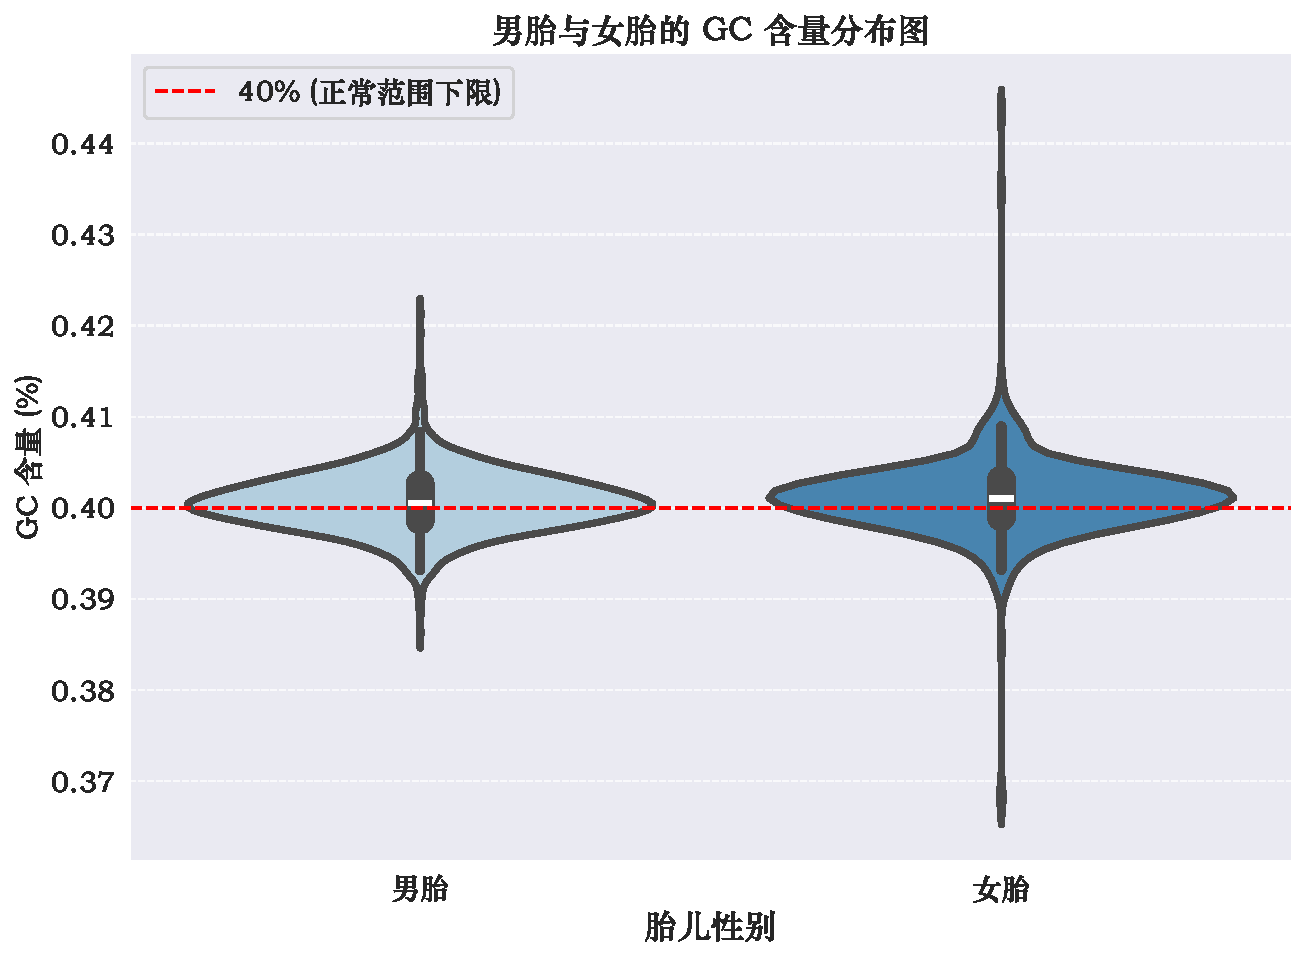
\includegraphics[width=0.8\textwidth]{chapters/数据预处理/images/数据清洗/GC值小提琴图.pdf}
    \caption{男胎与女胎的 GC 值小提琴图}
    \label{fig:violin}
\end{figure}

手动剔除分布不均匀的 $2$ 个 $GC < 0.39$ 的样本，以及 $2$ 个 $GC > 0.415$ 的样本，对于女胎样本，剔除分布不均匀的 $3$ 个 $GC < 0.39$ 的样本，以及 $2$ 个 $GC > 0.42$ 的样本。


\section{问题一的模型建立与求解}

本问求解流程如下：
\begin{figure} [H]
    \centering
    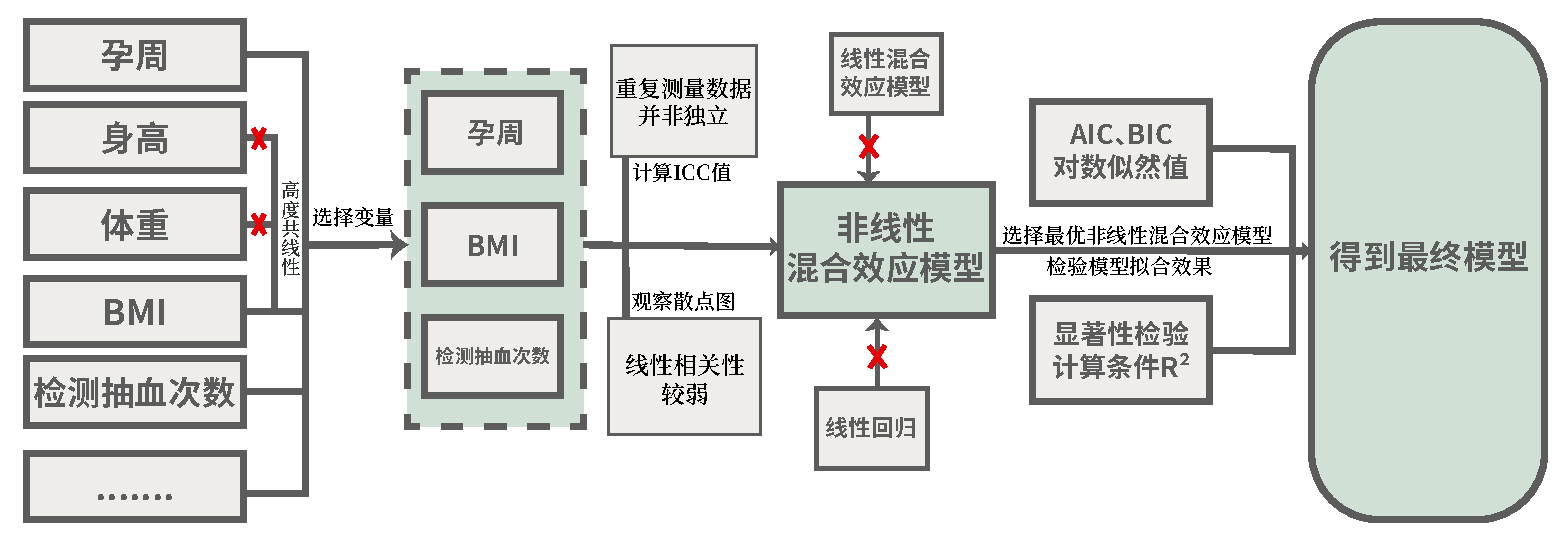
\includegraphics[width=\textwidth]{chapters/Q1/images/问题一的模型建立与求解/问题1流程图.pdf}
    \caption{问题1求解流程图}
    \label{fig:flowchart1}
\end{figure}

\subsection{符号说明}

为便于模型建立，本文对新增符号进行说明，其余符号沿用上文。

\begin{center}
    \begin{tabularx}{0.7\textwidth}{c@{\hspace{1pc}}|@{\hspace{2pc}}>{\centering\arraybackslash}X}
        \Xhline{0.08em}
        符号    & 符号说明               \\
        \Xhline{0.05em}
        $Y_i$ & 第 $i$ 个样本的 Y 染色体浓度 \\
        $c_i$ & 第 $i$ 个样本的检测抽血次数   \\
        \Xhline{0.08em}
    \end{tabularx}
\end{center}

\subsection{多重共线性分析与变量选择}

由于 BMI 可由身高体重得到，本文通过计算方差膨胀因子（VIF）以衡量这几个变量间的多重共线性程度。对于模型中的第 $i$ 个自变量，其 VIF 值的计算公式为：
$$
    \text{VIF}_i = \frac{1}{1 - R_i^2}
$$
其中，$R_i^2$ 是将自变量 $x_i$ 作为因变量，对数据集中所有其他自变量进行线性回归时所得到的决定系数。通常认为，当 $VIF > 10$ 时，模型存在严重的共线性问题。

计算可得，身高、体重与 BMI 三者存在多重共线性（如表 \ref{tab:vif_analysis} 所示，三个变量的 VIF 值均远大于 $10$），因此建模时仅选用 BMI 作为孕妇体型的代表指标。对于其他因素，图 \ref{fig:Y} 展示了多种孕妇因素与 Y 染色体浓度的散点图。

\begin{table}[H]
    \centering
    \caption{孕妇体重、身高与 BMI 的VIF值}
    \label{tab:vif_analysis}
    \begin{tabular}{ccc}
        \toprule
        \textbf{体重 VIF} & \textbf{孕妇BMI VIF} & \textbf{身高 VIF} \\
        \midrule
        360.38          & 224.34             & 109.31          \\
        \bottomrule
    \end{tabular}
\end{table}

\begin{figure} [H]
    \centering
    
\includegraphics[width=0.8\textwidth]{chapters/Q1/images/问题一的模型建立与求解/Y染色体浓度与有关系的变量的散点图.pdf}
    \caption{Y 染色体浓度与有关系的变量的散点图}
    \label{fig:Y}
\end{figure}

考虑到生产次数较多的孕妇与大龄产妇较少，在样本不足的情况下，无法确凿断定这两个因素对 Y 染色体浓度的影响。且随着生产次数的增多，Y 染色体浓度均值仍维持在 $0.08$ 左右，如表 \ref{tab:parity_Y} 所示：

\begin{table}[H]
    \centering
    \caption{按生产次数分组的 Y 染色体浓度均值}
    \label{tab:parity_Y}
    \begin{tabular}{c|cccc}
        \toprule
        \textbf{生产次数}      & 0      & 1      & 2      & 3      \\
        \midrule
        \textbf{Y 染色体浓度均值} & 0.0770 & 0.0759 & 0.0850 & 0.0789 \\
        \bottomrule
    \end{tabular}
\end{table}

若将 $a_i > 35$ 作为大龄产妇标准剔除，剔除前后其均值也几乎维持不变（全体样本：$0.07719$，剔除后：$0.07745$），仅相差 $0.34\%$，与散点图较为符合。因此本文认为：

\begin{itemize}[leftmargin=2em]
    \item 生产次数对 Y 染色体浓度不产生显著影响；
    \item 孕妇年龄对 Y 染色体浓度不产生显著影响；
\end{itemize}

除本文假设外，在一项针对超过两万名孕妇的大样本研究中\cite{zhou2015effects}，专门通过测量 Y 染色体来估算胎儿分数，其采用的模型如下：
\begin{equation}
    \varepsilon_{i,Y} = \frac{cr_{i,Y} - cr'_{i,Y,f}}{cr'_{i,Y,m} - cr'_{i,Y,f}}
    \label{eq:fetal_fraction}
\end{equation}
其中 $\varepsilon_{i,Y}$ 代表样本 $i$ 通过 Y 染色体估算出的胎儿分数。该研究明确指出，胎儿分数（即Y染色体浓度）与男胎母体年龄并无相关性，为本文的假设提供了有力支撑。

数据统计阶段可知，胎儿 Y 染色体浓度与大部分生理指标存在较弱的线性相关性。而由散点图（图 \ref{fig:Y}）可知，孕周、BMI 存在一定的正负相关性。离群散点较多，使用单纯的线性模型拟合效果不足。综合考虑下，本文选用探究\textbf{孕妇 BMI 值、孕周（或孕天数）与检测抽血次数}三个指标与 \textbf{Y 染色体浓度的非线性关系}。

\subsection{重复测量数据的非独立性}

考虑到数据中存在大量针对同一孕妇的重复测量记录，数据观测值之间并非相互独立，如对同一个样本进行多次的测量（如本题中的多次采血），该类数据被称为重复测量数据\cite{feng2020}。其特点是同一研究对象的重复测量值之间是非独立的。并且可能存在由于个体差异引起的相关性。传统的 $t$ 检验与方差分析，都要求数据具有独立性。

此类调查方式在生物医学研究中称为纵向研究。纵向研究与横断面研究有根本的区别。横断面研究是在个体只被观察一次的情况下进行的。然而，纵向研究关注于调查在不同时间上的变化，主要特征是研究对象在一段时间内被重复测量。

查找相关文献发现，混合效应模型（Mixed Effect Model）对同一统计单位进行重复测量或对相关统计单位集群进行测量的情况下有明显作用\cite{gomes2022should}，该模型能够将数据的变异区分为：代表普遍规律的固定效应和代表个体差异的随机效应\cite{gomes2022should}，进而可以得到更准确可靠的参数估计。

为定量验证采用混合效应模型的必要性，需首先计算Y染色体浓度达的组内相关系数（ICC）。ICC用于量化同一组\textbf{测量结果}之间的相关程度，在本题的情境下即同一孕妇的多个Y染色体浓度测量结果，其计算公式如下\cite{yu2022beyond}：
\begin{equation}
    \text{ICC} = \frac{\sigma_b^2}{\sigma_b^2 + \sigma_e^2}
\end{equation}
其中，$\sigma_b^2$ 表示组间方差，即不同孕妇之间的差异；$\sigma_e^2$ 表示组内方差，即同一孕妇的波动。ICC 的取值范围为 $0$ 到 $1$，如果 $ICC = 0$，则数据可视为不相关；如果 $ICC = 1$，则每个聚类中的所有观测值都完全相关。

Terry K. Koo 提出了检验 ICC 值的标准\cite{koo2016guideline}，具体如下：

\begin{itemize}[leftmargin=2em]
    \item $ICC < 0.5$，表示测量结果之间的相关性较差(原文为 Poor)；
    \item $0.5 \leq ICC < 0.75$，表示测量结果之间的相关性中等(原文为 Moderate)；
    \item $0.75 \leq ICC < 0.9$，表示测量结果之间的相关性良好(原文为 Good)；
    \item $ICC \geq 0.9$，表示测量结果之间的相关性极好(原文为 Excellent)。
\end{itemize}

\subsection{挑选最优非线性混合效应模型}

使用Python的 statsmodels 库对数据进行分析，计算得到 $ICC = 0.5984$，这说明同一孕妇的Y染色体浓度测量结果之间存在中等程度的相关性，所以混合效应模型在本题中是适用的。普通的非线性回归模型由于存在变量之间相互独立的假设，在本题中并不适用。因此，本文建立如下可能的非线性混合效应模型：
$$
    \begin{cases}
        Y = \beta_0 + \beta_1 w + \beta_2 w^2 + \beta_3 BMI + \beta_4 c                          & (a) \\
        Y = \beta_0 + \beta_1 w + \beta_2 w^2 + \beta_3 BMI + \beta_4 BMI^2 + \beta_5 c          & (b) \\
        Y = \beta_0 + \beta_1 w + \beta_2 w^2 + \beta_3 BMI + \beta_4 c + \beta_5 c^2            & (c) \\
        Y = \beta_0 + \beta_1 w + \beta_2 w^2 + \beta_3 BMI + \beta_4 c + \beta_5 (BMI \times w) & (d)
    \end{cases}
$$
其中，$Y$ 表示 Y 染色体浓度，$w$ 表示孕周数，$BMI$ 表示孕妇 BMI 值，$c$ 表示检测抽血次数，$\beta_i (i=0,1,2,\ldots)$ 为待估计的模型参数。

为了选择最优模型，本文使用赤池信息量准则（AIC）和贝叶斯信息量准则（BIC）作为模型评价指标。AIC和BIC均考虑了模型的拟合优度和复杂度，其值越小代表模型在解释数据和避免过拟合之间达到了更好的平衡。
AIC和BIC的计算公式如下：
\begin{numcases}
    \text{AIC} = 2k - 2\ln(L) \\
    \text{BIC} = k\ln(n) - 2\ln(L)
\end{numcases}

其中，$k$ 为模型参数的数量，$L$ 为模型的最大似然估计值，$n$ 为样本数量。计算结果如表 \ref{tab:model_comparison} 所示：

\begin{table}[H]
    \centering
    \caption{不同模型的比较结果}
    \label{tab:model_comparison}
    \begin{tabular}{lccc}
        \toprule
        \textbf{模型名称} & \textbf{AIC} & \textbf{BIC} & \textbf{对数似然值} \\
        \midrule
        模型\textit{a} & -5117.046702 & -5082.166662 & 2565.523351    \\
        模型\textit{c} & -5106.499492 & -5066.636590 & 2561.249746    \\
        模型\textit{b} & -5098.236333 & -5058.373431 & 2557.118166    \\
        模型\textit{d} & -5097.598194 & -5057.735292 & 2556.799097    \\
        \bottomrule
    \end{tabular}
\end{table}

由表 \ref{tab:model_comparison} 可知，模型 $a$ 的 AIC 和 BIC 值均为最小，且对数似然值最大，说明该模型在解释数据和避免过拟合之间达到了更好的平衡。因此，本文选择模型 $a$ 作为最终的非线性混合效应模型。
对模型$a$进行拟合，得到如下结果：

\begin{table}[H]
    \centering
    \caption{模型的拟合结果}
    \label{tab:model_fit}
    \begin{tabular}{l c c c c c c}
        \toprule
                                        & \textbf{Coef.} & \textbf{Std.Err.} & \textbf{z} & \textbf{P>|z|} & \multicolumn{2}{c}{\textbf{[0.025 0.975]}}          \\
        \midrule
        \textbf{Intercept}              & 0.218          & 0.020             & 10.705     & 0.000          & 0.178                                      & 0.258  \\
        \textbf{孕周}                     & -0.012         & 0.002             & -7.880     & 0.000          & -0.015                                     & -0.009 \\
        \textbf{孕周 \textsuperscript{2}} & 0.000          & 0.000             & 8.598      & 0.000          & 0.000                                      & 0.000  \\
        \textbf{孕妇BMI}                  & -0.002         & 0.000             & -4.290     & 0.000          & -0.003                                     & -0.001 \\
        \textbf{检测抽血次数}                 & 0.012          & 0.001             & 10.936     & 0.000          & 0.010                                      & 0.014  \\
        \bottomrule
    \end{tabular}
\end{table}

由于表 \ref{tab:model_fit} 中的数据会进行四舍五入，导致部分数字显示为 $0.000$。为检验\textbf{显著性水平}，Statsmodels库在构建此模型时会同步进行沃尔德检验，其核心思想在于评估参数的点估计值与其标准误差的比值：对于模型中的每一个参数 $\beta_j$，本文首先设立原假设 $H_0: \beta_j=0$，即该变量对因变量没有影响。随后计算 $z$ 统计量：
\begin{equation}
    z = \frac{\hat{\beta}_j}{\text{SE}(\hat{\beta}_j)}
\end{equation}
其中，$\hat{\beta}_j$ 是参数 $\beta_j$ 的最大似然估计值，$\text{SE}(\hat{\beta}_j)$ 是其对应的标准误差。在原假设成立的条件下，该 $z$ 统计量近似服从标准正态分布。

基于此，本文的详细检验结果已在表 \ref{tab:pvalues} 中呈现，所有变量的 $p$ 值均远小于 0.05，证明了其高度的统计显著性。

\begin{table}[H]
    \centering
    \caption{回归系数表}
    \label{tab:coefficients}
    \begin{tabular}{lccccc}
        \toprule
        \textbf{变量}         & \textbf{Intercept} & \textbf{孕周} & \textbf{孕周$^2$} & \textbf{孕妇BMI} & \textbf{检测抽血次数} \\
        \midrule
        \textbf{系数 (Coef.)} & 0.218290           & -0.011993   & 0.000326        & -0.002045      & 0.012028        \\
        \bottomrule
    \end{tabular}
\end{table}

\begin{table}[H]
    \centering
    \caption{显著性水平表}
    \label{tab:pvalues}
    \begin{tabular}{lccccc}
        \toprule
        \textbf{变量}         & \textbf{Intercept} & \textbf{孕周}  & \textbf{孕周$^2$} & \textbf{孕妇BMI} & \textbf{检测抽血次数} \\
        \midrule
        \textbf{p值 (P>|z|)} & 9.601115e-27       & 3.262814e-15 & 8.078243e-18    & 1.784269e-05   & 7.727184e-28    \\
        \bottomrule
    \end{tabular}
\end{table}

由表 \ref{tab:coefficients} 可知，在混合效应模型中，各变量的系数均不为零，孕周与孕妇BMI与Y染色体浓度呈负相关，而孕周平方与检测抽血次数则与Y染色体浓度呈正相关。由表 \ref{tab:pvalues} 可知，所有变量的 $p$ 值均远小于 $0.05$，说明在统计学上均显著影响 Y 染色体浓度，通过显著性检验。
此前的研究已普遍发现：胎儿 DNA 浓度随孕龄增加而增加，随孕妇体重增加而减少。因此，本文构建的最终的非线性混合效应模型为：
\begin{equation}
    Y = 0.218290 - 0.011993 w + 0.000326 w^2 - 0.002045 BMI + 0.012028 c \label{eq:final_model}
\end{equation}
其中，$Y$ 表示 Y 染色体浓度，$w$ 为孕周数，$c$ 表示检测抽血次数。

从统计学角度看，文献中的发现也与本模型的变量显著性结论一致。研究明确指出，孕周与 Y 染色体浓度的相关性 ($P<.001$) 以及孕妇 BMI 与其的相关性 ($P<.001$) 均达到了统计学上的高度显著水平\cite{zhou2015effects}。这表明将孕周、孕周的二次方以及孕妇 BMI 纳入模型是合理且必要的。

本文还对模型的条件 $R^2$ 值进行了计算，以评估模型的解释力。条件 $R^2$ 值考虑了固定效应和随机效应的贡献，其计算公式为：
\begin{equation}
    R^2_c = \frac{\sigma_f^2 + \sigma_r^2}{\sigma_f^2 + \sigma_r^2 + \sigma_e^2}
    \label{eq:conditional_r2}
\end{equation}
其中，$\sigma_f^2$ 表示固定效应的方差，$\sigma_r^2$ 表示随机效应的方差，$\sigma_e^2$ 表示残差的方差。

计算得到模型的条件 $R^2$ 值为 $0.7664$，说明模型能够解释约 $76.64\%$ 的 Y 染色体浓度的变异。本文也将模型的拟合效果可视化，如图 \ref{fig:model_fit} 所示：
\begin{figure}[H]
    \centering
    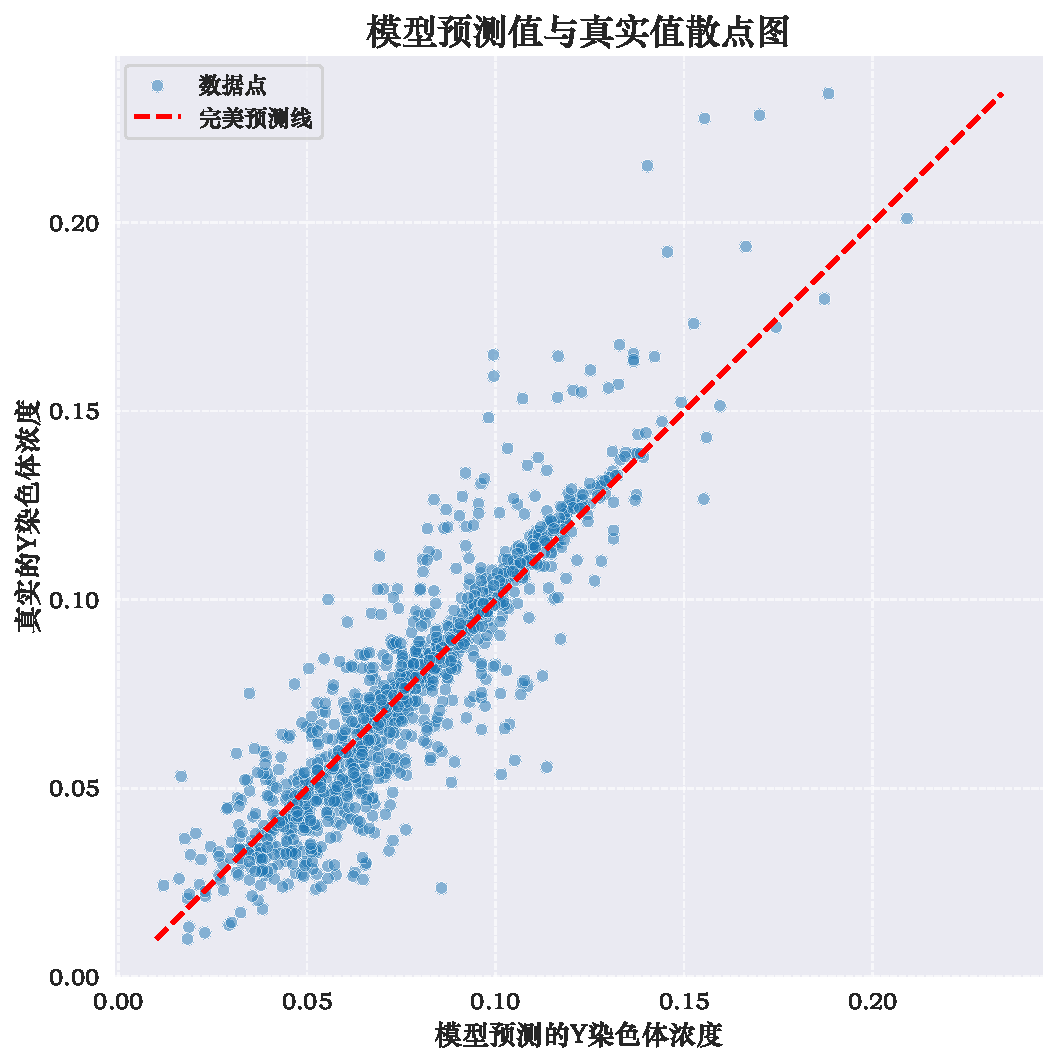
\includegraphics[width=0.6\textwidth]{chapters/Q1/images/问题一的模型建立与求解/预测值与真实值.pdf}
    \caption{模型的拟合效果图}
    \label{fig:model_fit}
\end{figure}

综上，对于问题一，本文综合考虑孕妇 BMI 值、孕周与检测抽血次数三个指标，建立了一个非线性混合效应模型来描述这些因素与 Y 染色体浓度之间的关系。通过模型选择和评估，最终确定了模型 $a$ 作为最优模型，拟合出的模型系数也呈现出极强的显著性。此外，模型的条件 $R^2$ 值为 $0.7664$，说明该模型具有较强的解释力，能够较好地反映孕妇相关因素对 Y 染色体浓度的影响。


\section{问题二的模型建立与求解}

\subsection{符号说明}

\begin{center}
    \begin{tabularx}{0.8\textwidth}{c@{\hspace{1pc}}|@{\hspace{2pc}}>{\centering\arraybackslash}X}
        \Xhline{0.08em} % 表格顶部粗线
        \textbf{符号} & \textbf{符号说明}            \\
        \Xhline{0.05em}
        $R_i$       & 第 $i$ 个样本“染色体的非整倍体”的检测结果 \\
        $P_i$       & 第 $i$ 个样本预测的“胎儿是否健康”结果   \\
        $H_i$       & 第 $i$ 个样本“胎儿是否健康”的实际情况记录 \\
        $E_i$       & 对第 $i$ 个样本预测准确性的最终评估结果   \\
        \Xhline{0.08em}
    \end{tabularx}
\end{center}

本文建立了评估结果指标 $E_i$ 通过比较预测值 $P_i$ 和实际值 $H_i$ 来确定。如果两者相等，则评估为“准确”；如果不相等，则为“不准确”。
本文可以用一个决策函数来表示：
\begin{equation}
    P_i =
    \begin{cases}
        1 & ,R_i \text{为空} \\
        0 & ,R_i \text{非空}
    \end{cases}
    \quad \quad
    H_i =
    \begin{cases}
        1 & ,\text{“是”} \\
        0 & ,\text{“否”}
    \end{cases}
    \quad \quad
    E_i =
    \begin{cases}
        1 & ,P_i = H_i    \\
        0 & ,P_i \neq H_i
    \end{cases}
\end{equation}

\begin{center}
    \begin{tabularx}{0.8\textwidth}{c@{\hspace{1pc}}|@{\hspace{2pc}}>{\centering\arraybackslash}X}
        \Xhline{0.08em} % 表格顶部粗线
        \textbf{符号}  & \textbf{符号说明（续表）}                                                \\
        \Xhline{0.05em}
        $B$          & BMI分组的边界点向量                                                      \\
        $R(w)$       & 孕周为 $w$ 时的潜在风险函数                                                 \\
        $S_j$        & 第 $j$ 组 ($G_j$) 内的样本集合                                           \\
        $S_{j,w}$    & 第 $j$ 组在孕周窗口 $[w, w+1)$ 内的样本子集                                   \\
        $N_{j,w}$    & 窗口样本数, 即 $|S_{j,w}|$                                             \\
        $A(S_{j,w})$ & 窗口 $S_{j,w}$ 内的检测成功率                                             \\
        $w_j^*$      & 第 $j$ 组的最佳NIPT时点 (孕周)\footnote{在优化理论中，上标星号（*）通常用来表示最优解。另外的符号同理。} \\
        \Xhline{0.08em}
    \end{tabularx}
\end{center}

\subsection{模型假设}

基于题干对探究 BMI 范围与 NIPT 检测时点的关系的要求，本文做出以下假设：

\begin{enumerate}
    \item 假设孕妇的BMI是影响胎儿Y染色体浓度达标时间的主要因素，其他因素可暂时视为次要影响或随机扰动。
    \item 假设风险与孕周的阶梯关系可量化，且风险值随孕周增加而递增。
\end{enumerate}

\subsection{数据分析}

由于男胎的 Y 染色体浓度达到或高于 4\% 才被认为 NIPT 的结果是基本正确的，为了给出每组的 BMI 区间和最佳 NIPT
时点，本文在进行求解前，探究了对男胎孕妇 BMI 与孕周数之间的关系，Y 染色体浓度小于 4\% 的散点被标注出来。同时，孕妇代码 A160 的 BMI 值偏低（$20.7$），视作离群点，不具统计意义，剔除后，分布如图 \ref{fig:BMI 与孕周散点图} 所示：

\begin{figure} [H]
    \centering
    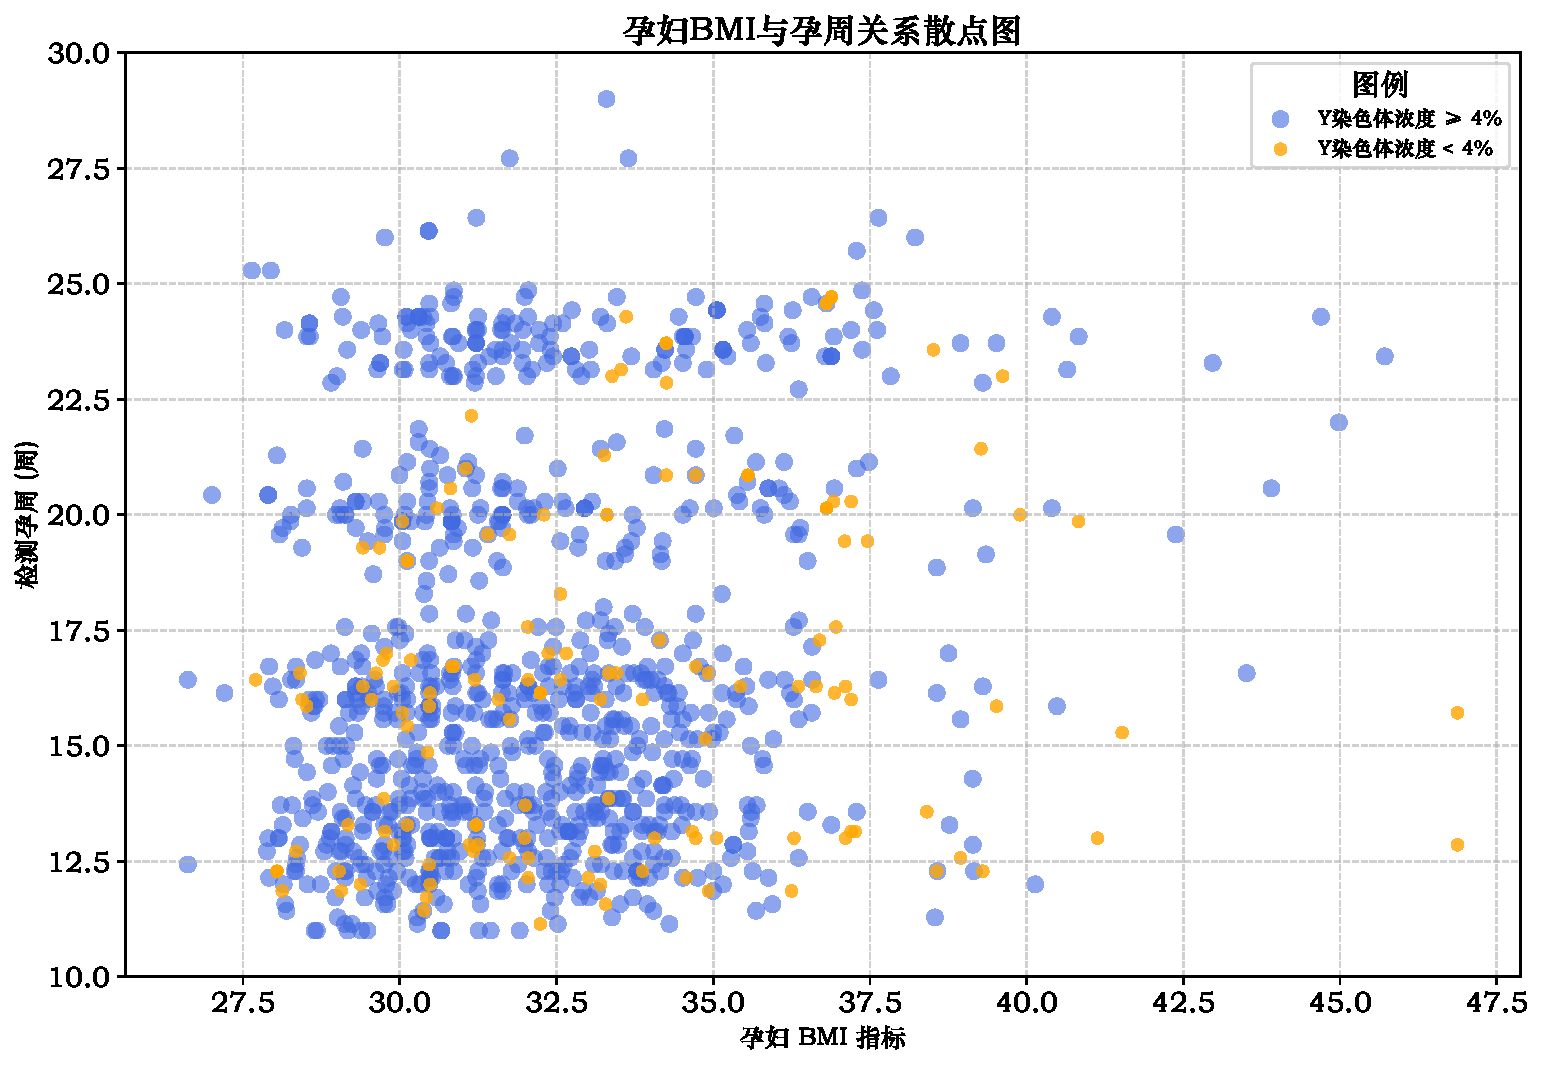
\includegraphics[width=0.7\textwidth]{chapters/Q2/images/BMI 与孕周散点图.pdf}
    \caption{BMI 与孕周散点图}
    \label{fig:BMI 与孕周散点图}
\end{figure}

同时，本文根据上述模型，以红色标注出 NIPT 检验结果不准确的样本（即 $E_i = 0$ 的样本点），分布如图 \ref{fig:检验结果不准确} 所示：

\begin{figure} [H]
    \centering
    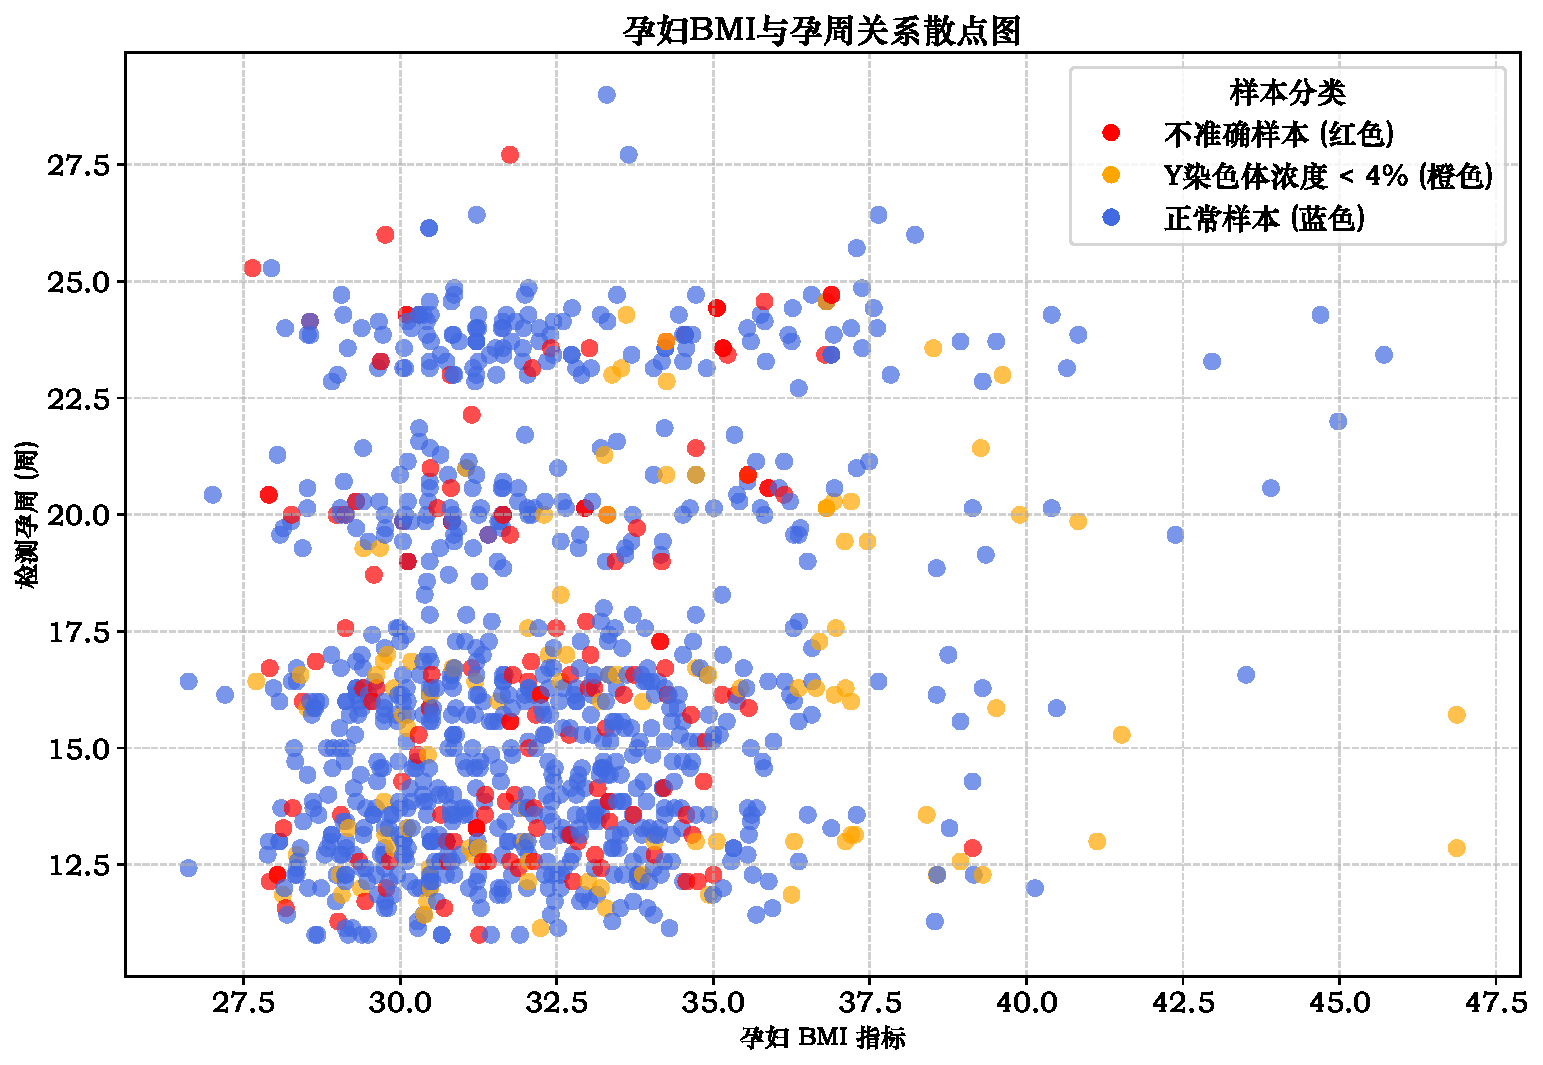
\includegraphics[width=0.7\textwidth]{chapters/Q2/images/标注全部不准确散点图.pdf}
    \caption{检验结果不准确的样本散点图}
    \label{fig:检验结果不准确}
\end{figure}

\subsection{K-Means 算法选择聚类数量}

K-Means 算法预先指定初始聚类数以及初始化聚类中心，按照样本之间的距离大小，把样本集根据数据对象与聚类中心之间的相似度划分为类簇，不断更新聚类中心的位置，不断降低类簇的误差平方和，当 SSE 不再变化或目标函数收敛时，聚类结束，得到最终结果。

\newpage

\begin{enumerate}
    \item 先从数据集中随机选取K个初始聚类中心 $C_j(1 \leq j \leq k)$ ，计算其余数据对象与聚类中心 $C_j$ 的欧氏距离，找出离目标数据对象最近的聚类中心 $C_j$ ，并将数据对象分配到聚类中心 $C_j$ 所对应的簇中；
    \item 接着计算每个簇中数据对象的平均值，将该值当作新的聚类中心，进行下一次迭代，直到聚类中心不再变化或达到最大的迭代次数时停止。
\end{enumerate}

空间中数据对象与聚类中心间的欧氏距离计算公式为：
\begin{equation}
    d\left(X, C_j\right)=\sqrt{\sum_{d=1}^m\left(X_d-C_{j d}\right)^2}
\end{equation}
其中，$X$ 为数据对象；$C_i$ 为第 $i$ 个聚类中心；$m$ 为数据对象的维度；$X_j$、$C_{ij}$ 为 $X$ 和 $C_i$ 的第 $j$ 个属性值。整个数据集的 SSE 计算公式为：
\begin{equation}
    \mathrm{SSE}=\sum_{j=1}^k \sum_{X \in C_j}\left|d\left(X, C_j\right)\right|^2
\end{equation}
其中，SSE 的大小表示聚类结果的好坏；$k$ 为簇的个数。
K-Means 的本质是通过迭代最小化 SSE 实现聚类，默认距离使用欧氏距离。其算法流程图如下所示：
\begin{figure} [H]
    \centering
    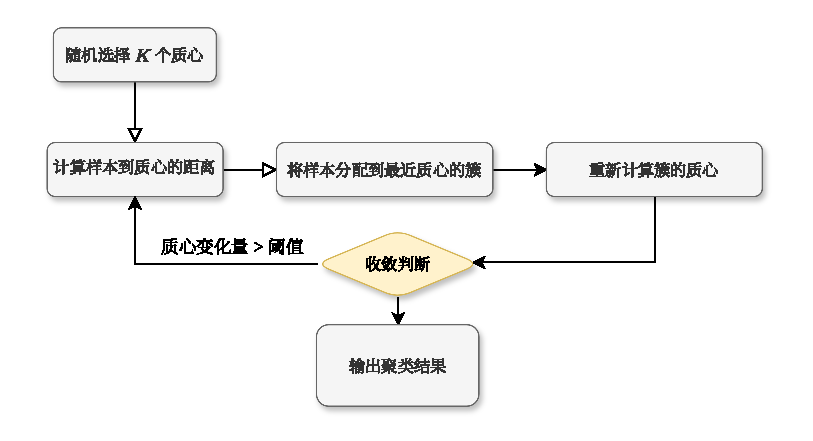
\includegraphics[width=0.65\textwidth]{chapters/Q2/images/KMeans-Drawio.pdf}
    \caption{K-Means 算法流程图}
\end{figure}

本文使用肘部法则确定最优聚类数 $K$。肘部法通过计算不同 $K$ 值下的 SSE，绘制 SSE 随 $K$ 变化的曲线图，选择曲线出现“肘部”位置对应的 $K$ 值作为最优聚类数。绘制的肘部法曲线图如 \ref{fig:K-Means手肘法} 所示。观察图 \ref{fig:K-Means手肘法} 可知，当 $k = 2,3,4$ 时都是可考虑的值。为了让不同 BMI 的孕妇能够获得更精细的 NIPT 检测时点建议，并且也与题干给出的分组组数相似，故本文选择 $k=4$ 作为最终的聚类数。

\begin{figure}[H]
    \centering
    \begin{minipage}{0.48\textwidth}
        \centering
        
\includegraphics[width=\textwidth]{chapters/Q2/images/K-Means手肘法.pdf}
        \caption{K-Means手肘法}
        \label{fig:K-Means手肘法}
    \end{minipage}
    \hfill
    \begin{minipage}{0.48\textwidth}
        \centering
        
\includegraphics[width=\textwidth]{chapters/Q2/images/BMI聚类分析结果.pdf}
        \caption{BMI聚类分析结果}
        \label{fig:BMI聚类分析结果}
    \end{minipage}
\end{figure}

图 \ref{fig:BMI聚类分析结果} 展示了散点图的聚类结果，并且用红线标注了聚类的中心点，从中本文可以看出，聚类效果较好，且各个簇之间的间隔较大，说明不同 BMI 的孕妇在 NIPT 检测时点上可能存在显著差异。

\subsection{多目标优化}

\subsubsection{潜在风险函数}

据题意，本文将不同孕周的潜在风险定义为一个分段函数。早期（$12$周及以内）风险低；中期（$13 \sim 27$周）风险随孕周线性增高；晚期（$28$周及以后）风险极高。具体函数如下：
\begin{equation}
    R(w) =
    \begin{cases}
        1                      & ,\text{若}\ \ w \le 12        \\
        10 + 3 \times (w - 13) & ,\text{若}\ \ 13 \le w \le 27 \\
        100                    & ,\text{若}\ \ w \ge 28
    \end{cases}
    \label{eq:risk_function}
\end{equation}

\subsubsection{加权和法确定目标函数}

寻找最佳的 BMI 区间的核心目标是最小化孕妇的潜在风险，同时最大化采样检测的准确率。通过加权和法，本文将此多目标问题转化为单目标优化问题。目标是寻找一组最优的 BMI 边界点 $B^*$，使得加权的总体目标函数 $F(B)$ 最小。
\begin{equation}
    B^* = \arg\min_{B} F(B)
    \label{eq:optimization_goal}
\end{equation}

\paragraph*{最小化总体潜在风险}

第一个目标是使所有孕妇的平均潜在风险最低。对于一组给定的BMI边界点 $B$，本文可以为每个分组 $G_i$ 找到其最佳检测孕周 $w_i^*$。该分组内所有样本的风险均按 $R(w_i^*)$ 计算。因此，全体样本的加权平均风险 $F_{risk}(B)$ 可以表示为：
\begin{equation}
    \min F_{risk}(B) = \min \left( \frac{\sum_{j=1}^{4} |S_j| \cdot R(w_j^*)}{\sum_{j=1}^{4} |S_j|} \right)
    \label{eq:risk_objective}
\end{equation}
其中 $|S_i|$ 是第 $i$ 组的样本总数，作为权重，以确保样本量大的分组在总体风险评估中占有相应比重。

\paragraph*{最大化总体检测准确率}

第二个目标是使在推荐窗口内进行检测的样本，其总体准确率最高。准确率 $A(S_{i, w_i^*})$ 定义为在第 $i$ 组的最佳窗口 $S_{i, w_i^*}$ 内，检测成功（Y染色体浓度达标且结果准确）的样本比例。总体加权平均准确率 $F_{acc}(B)$ 可以表示为：
\begin{equation}
    \max F_{acc}(B) = \max \left( \frac{\sum_{j=1}^{4} |S_{j, w_j^*}| \cdot A(S_{j, w_j^*})}{\sum_{j=1}^{4} |S_{j, w_j^*}|} \right)
    \label{eq:accuracy_objective}
\end{equation}
其中 $|S_{j, w_j^*}|$ 是推荐窗口内的样本数，作为权重。

\paragraph*{从多目标优化转为单目标优化}

标准的优化算法通常只能处理单一方向（例如求最小值）的问题。本文选择将所有目标统一为\textbf{最小化}。这是由于 minimize 模块是为最小化定制的。对于``最大化准确率"($F_{acc}$)，本文将其等价于\textbf{最小化不准确率}，即 $1 - F_{acc}$，再使用经典的“加权和法”将这两个最小化目标合并为一个单一的、综合的函数 $F(B)$。通过为每个目标分配一个权重（$w_{risk}$ 和 $w_{acc}$），以确保潜在风险最小为首要任务，可人工赋予权重 $w_{risk} = 0.7 > w_{acc} = 0.3$。最终的优化目标可以表示为：
\begin{equation}
    B^* = \arg\min_{B} F(B)
    \label{eq:optimization_goal}
\end{equation}
其中，总体目标函数 $F(B)$ 定义为所有分组的加权风险与加权不准确率之和：
\begin{equation}
    F(B) = w_{risk} \cdot F_{risk}(B) + w_{acc} \cdot \left( 1 - F_{acc}(B) \right)
    \label{eq:objective_function_final}
\end{equation}

\subsubsection{约束条件}

为了确保模型解的合理性和统计有效性，优化过程必须满足以下约束条件：

\begin{enumerate}
    \item \textbf{边界点单调性}: 为了保证BMI分组的逻辑正确性，分为四组需 5个边界点 $b_i$，满足单调递增关系，即 $b_i < b_{i+1}$，其中 $i = 1, 2, 3, 4$。

    \item \textbf{推荐窗口宽度}: 考虑到临床操作的灵活性和单周样本量的稀疏性问题，本文将NIPT推荐时间窗口的宽度设定为\textbf{两周}。例如，若推荐起始周为 $w_i^*$，则对应的窗口为 $[w_i^*, w_i^*+2)$。

    \item \textbf{窗口样本量约束}: 为了保证所选窗口的成功率计算具有统计学意义，同时避免结果被样本量异常集中的窗口所主导，本文对窗口内的样本数量 $N_{j, w_j^*}$ 设定了上下限。在本模型中，本文设定最小样本数为 $50$，最大样本数为 $100$。
          \begin{equation}
              50 \le N_{j, w_j^*} = |S_{j, w_j^*}| \le 100, \quad \forall j \in \{1, 2, 3, 4\}
              \label{eq:constraint_new}
          \end{equation}
\end{enumerate}

本文采用 Python 中的 scipy.optimize.minimize 库，基于序列最小二乘规划（SLSQP）求解器对目标函数进行迭代优化，寻找最优的 BMI 边界点。
为了提高优化效率，使用 BMI 的 $0, 25, 50, 75, 100$ 百分位点作为初始边界点（如图 \ref{fig:BMI四分位点}）。

\begin{figure} [H]
    \centering
    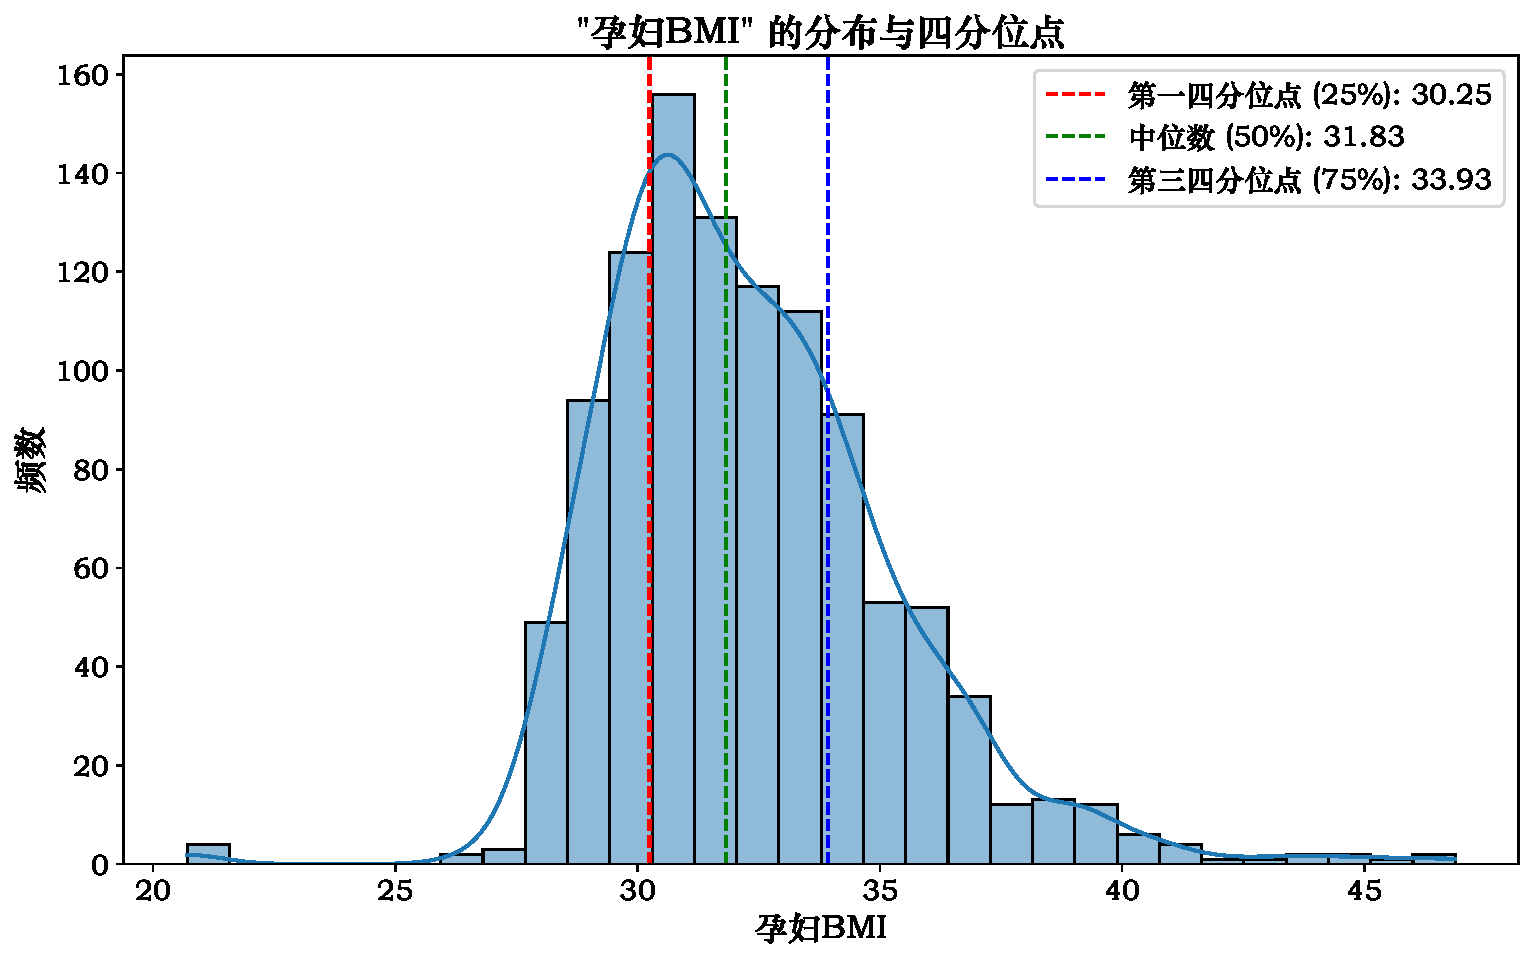
\includegraphics[width=0.6\textwidth]{chapters/Q2/images/孕妇BMI的四分位点.pdf}
    \caption{孕妇BMI的四分位点}
    \label{fig:BMI四分位点}
\end{figure}

经优化，本文得到的最优 BMI 分组方案及对应的最佳 NIPT 时点建议如表 \ref{tab:results} 所示。

\begin{table}[H]
    \centering
    \caption{最优BMI分组及NIPT时点推荐方案}
    \label{tab:results}
    \begin{tabular}{ccccc}
        \toprule
        \textbf{BMI分组} & \textbf{BMI区间} & \textbf{最佳NIPT时点 (周)} & \textbf{窗口内样本数} & \textbf{窗口内成功率} \\
        \midrule
        分组 1           & [26.62, 30.28) & 13 -- 15              & 60              & 85.00\%         \\
        分组 2           & [30.28, 31.88) & 15 -- 17              & 58              & 77.59\%         \\
        分组 3           & [31.88, 33.95) & 14 -- 16              & 52              & 90.38\%         \\
        分组 4           & [33.95, 46.87) & 15 -- 17              & 59              & 69.49\%         \\
        \bottomrule
    \end{tabular}
\end{table}

\v{-1em}

为直观验证上述优化方案的有效性，本文将表 \ref{tab:results} 中得到的四个最优 NIPT 推荐窗口，以高亮矩形区域的形式叠加绘制在原始的散点图上，结果如 \ref{fig:BMI分组和最佳NIPT时点} 所示。推荐窗口精确地覆盖了正常样本（蓝色点）的密集区域，同时有效规避了不准确样本（红色点）和Y染色体浓度过低样本（橙色点）的集中分布区。这种直观的对应关系，证实了该模型在平衡检测成功率与潜在风险两方面的优越性。

\begin{figure} [H]
    \centering
    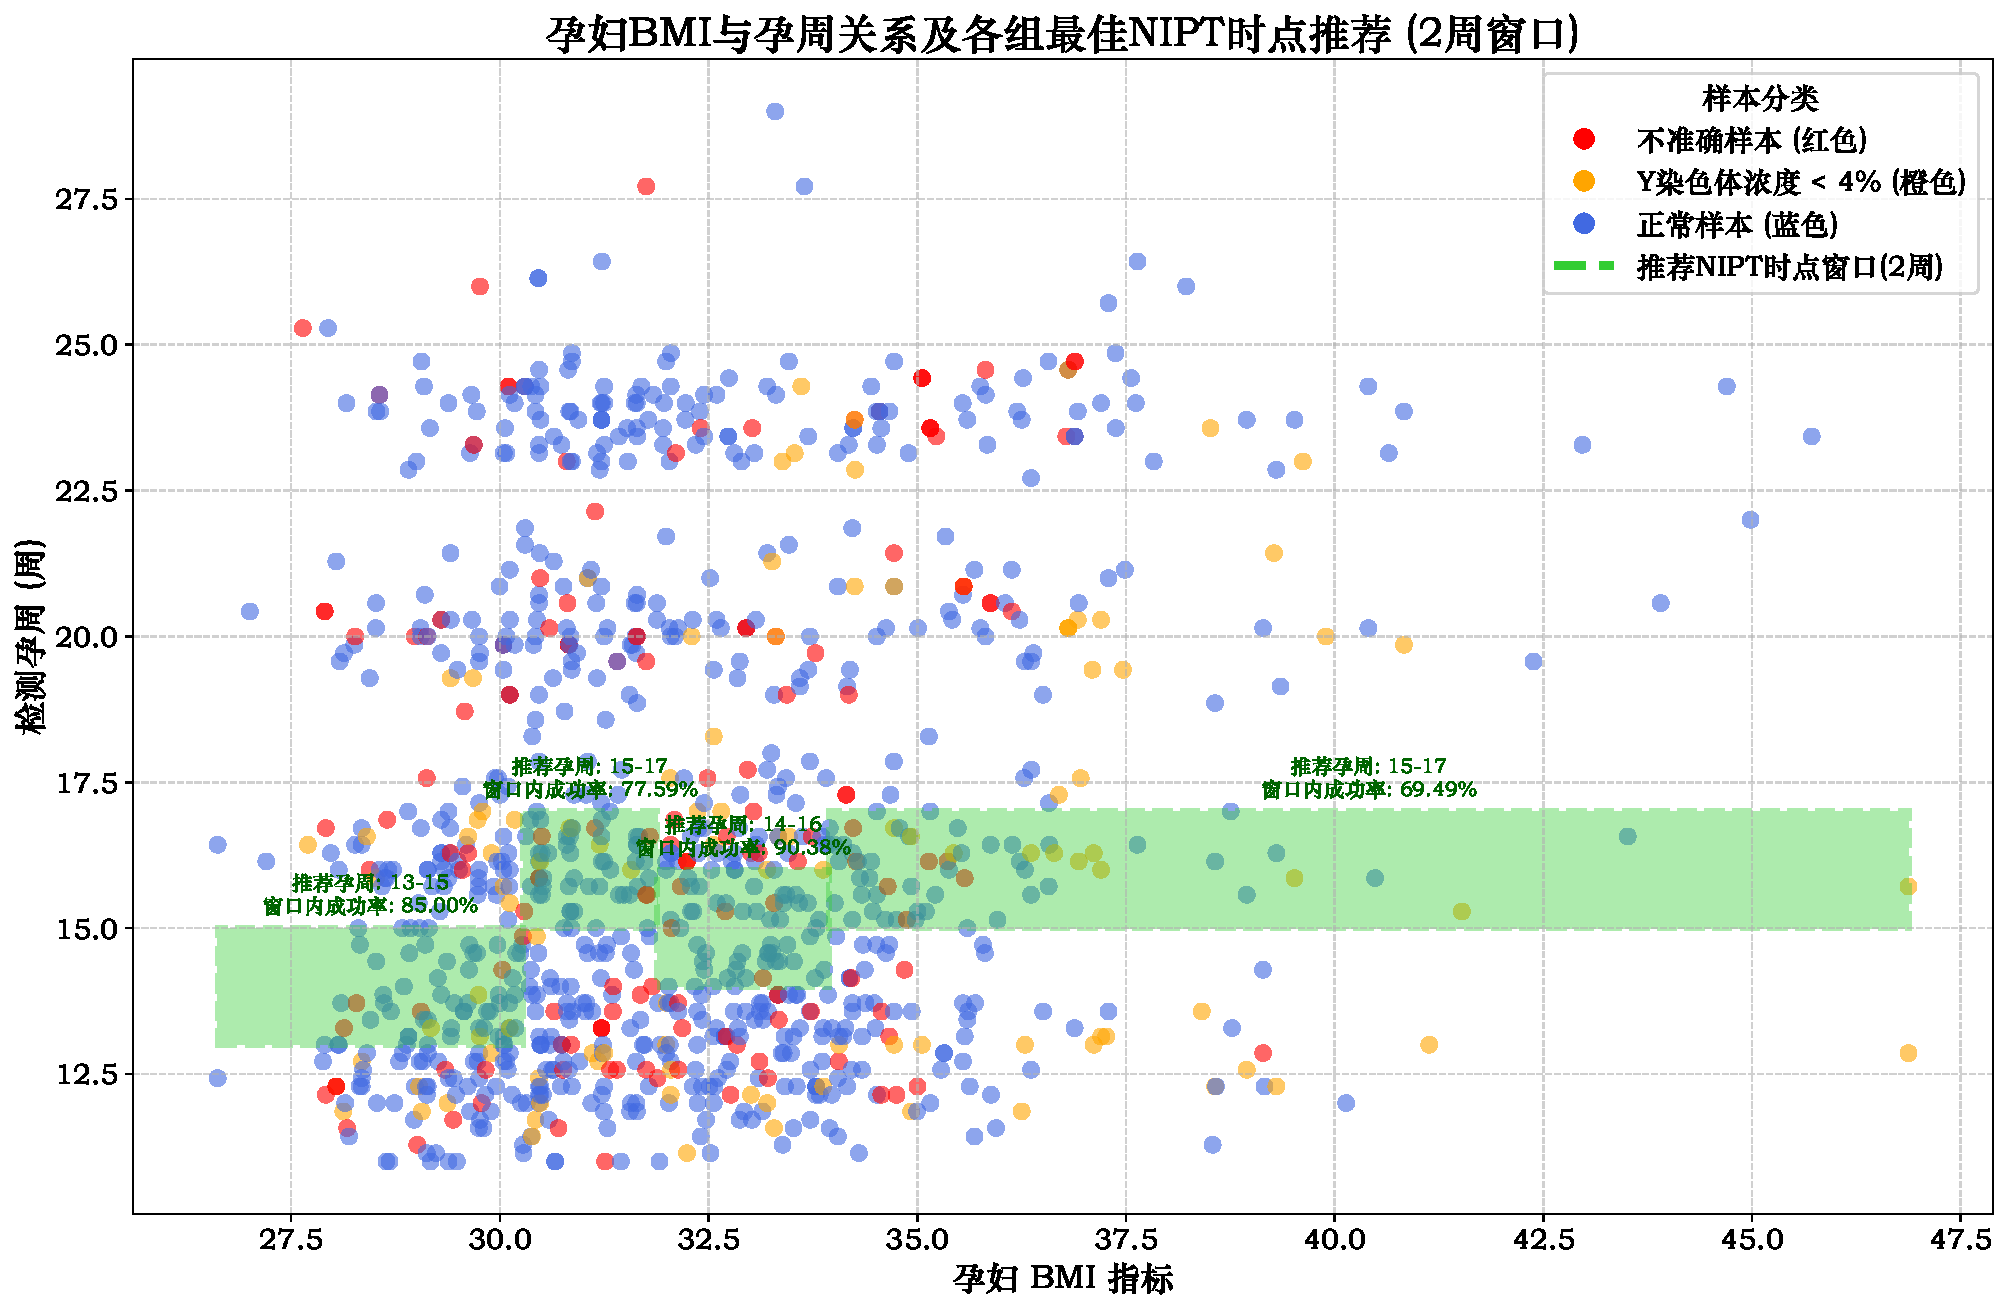
\includegraphics[width=0.75\textwidth]{chapters/Q2/images/BMI分组和最佳NIPT时点.pdf}
    \caption{BMI分组和最佳NIPT时点}
    \label{fig:BMI分组和最佳NIPT时点}
\end{figure}

表 \ref{tab:results} 将孕妇 BMI 值划分为四个亚组，其合理性在于借鉴了临床通用的 BMI 四分类标准（偏瘦、正常、超重、肥胖）思想\cite{WHO2005SuRF}，实现了对高风险人群的内部精细化分层。孕期母体为支持胎儿生长、胎盘发育及增加血容量等生理需求，体重和 BMI 必然显著增加\cite{kominiarek2017gestational}。该方案为不同 BMI 区间的孕妇提供了精确、可靠的 NIPT 检测时间窗口建议。所有推荐窗口均基于超过 $50$ 个样本的数据得出，保证了结论的统计稳健性。不仅如此，通过敏感性分析证实，当模型中的权重系数在 20\% 的容差范围内浮动时，最终得出的最优分组方案与时点建议均保持不变，充分证明了该决策模型的参数稳健性。由于过高或过低的 BMI 样本较少，本文模仿四分类标准，为男胎孕妇提供更具普适性的 BMI 与 NIPT 检测时间窗口建议（于表 \ref{tab:optimized_nipt_schedule}）。

\begin{table}[H]
    \centering
    \caption{基于BMI分层的NIPT最佳时点推荐方案}
    \label{tab:optimized_nipt_schedule}
    \begin{tabular}{cc}
        \toprule
        \textbf{BMI范围}           & \textbf{推荐NIPT最佳检测孕周} \\
        \midrule
        $BMI < 30.28$            & $13 \sim 15$ 周        \\
        $30.28 \leq BMI < 31.88$ & $15 \sim 17$ 周        \\
        $31.88 \leq BMI < 33.95$ & $14 \sim 16$ 周        \\
        $33.95 \leq BMI$         & $15 \sim 17$ 周        \\
        \bottomrule
    \end{tabular}
\end{table}

\begin{center}
    \begin{tikzpicture}
        % 绘制带箭头的数轴，并标记为 BMI
        \draw[->, thick] (0,0) -- (12,0) node[right] {BMI};

        % --- 定义关键坐标点 ---
        % 这里我们将 BMI 的范围映射到 x 轴的 0-12 范围内以便于绘图
        \def\pointOne{3.5}   % 对应 BMI 30.28
        \def\pointTwo{6}     % 对应 BMI 31.88
        \def\pointThree{9}   % 对应 BMI 33.95

        % --- 标记数轴上的关键点 ---
        % 绘制小圆点并在线下方标记数值
        \draw (\pointOne, 0) circle (2pt) node[below=4pt] {$30.28$};
        \draw (\pointTwo, 0) circle (2pt) node[below=4pt] {$31.88$};
        \draw (\pointThree, 0) circle (2pt) node[below=4pt] {$33.95$};

        % --- 在数轴上方绘制分段大括号并标注推荐孕周 ---
        % amplitude=10pt 控制了大括号的"胖瘦"，值越大，括号越大
        % above=15pt 控制了括号上方文字的距离
        \draw [decorate, decoration={brace, amplitude=10pt}]
        (0,0) -- (\pointOne,0)
        node [midway, above=15pt] {$13 \sim 15$ 周};

        \draw [decorate, decoration={brace, amplitude=10pt}]
        (\pointOne,0) -- (\pointTwo,0)
        node [midway, above=15pt] {$15 \sim 17$ 周};

        \draw [decorate, decoration={brace, amplitude=10pt}]
        (\pointTwo,0) -- (\pointThree,0)
        node [midway, above=15pt] {$14 \sim 16$ 周};

        \draw [decorate, decoration={brace, amplitude=10pt}]
        (\pointThree,0) -- (12,0)
        node [midway, above=15pt] {$15 \sim 17$ 周};

    \end{tikzpicture}
\end{center}

为探究孕妇 BMI 对所需孕周 $w$ 的影响，本文据问题一中构建的模型（见式 \ref{eq:final_model}）进行分析。在保持 Y 值与协变量检测次数 $c$ 恒定的条件下，对该式进行移项可得：
\begin{equation}
    Y - 0.218290 - 0.012028c + 0.002045 \cdot BMI = 0.000326w^2 - 0.011993w
\end{equation}

等式左侧是随 BMI 值单调递增的线性函数。为维持等式成立，等式右侧关于 $w$ 的二次函数 $f(w) = 0.000326w^2 - 0.011993w$ 的值也必须相应增大。该二次函数在 $w > 18.39$ 的区间内为增函数，符合本文中 $w$（孕周）的实际取值范围。在其他条件不变时，BMI 越高的孕妇，需要越长的孕周（即越大的 $w$ 值）才能达到相同的 $Y$ 值。BMI 越高的孕妇群体，其 Y 染色体浓度达到 $4\%$ 标准所需的孕周越长（即越大的 $w$ 值），在权衡检测准确度和潜在风险的前提下，建议的 NIPT 时点也相应推迟，与本文表 \ref{tab:optimized_nipt_schedule} 中的高 BMI 推荐最佳检测孕周相对应。

\subsection{模型有效性与检测误差分析}

在本文的数据情境下，“检测误差”由可观测的两种不良检测样本点构成，即检测不准确点（红色）与检测失败点（橙色，男胎Y染色体浓度低于4\%，导致本次检测不可靠）。检测失败常要求孕妇重新检测，增加成本、延长诊断时间，无疑会增加孕妇及其家庭的焦虑，并压缩了后续可能的医疗干预窗口。

为评估本模型规避检测误差的效果，本文采用\textbf{组内对比分析}方法，将当前推荐的最佳NIPT窗口内的成功率，与该分组自身的所有样本的平均成功率进行比较。

\subsubsection{组内成功率对比}

在模型根据全局目标函数（公式 \ref{eq:objective_function_final}）找到最优的BMI边界点后，本文对划分出的四个孕妇群体进行组内分析。详细的对比数据如图 \ref{fig:组内检测成功率对比图} 所示。

\begin{figure} [H]
    \centering
    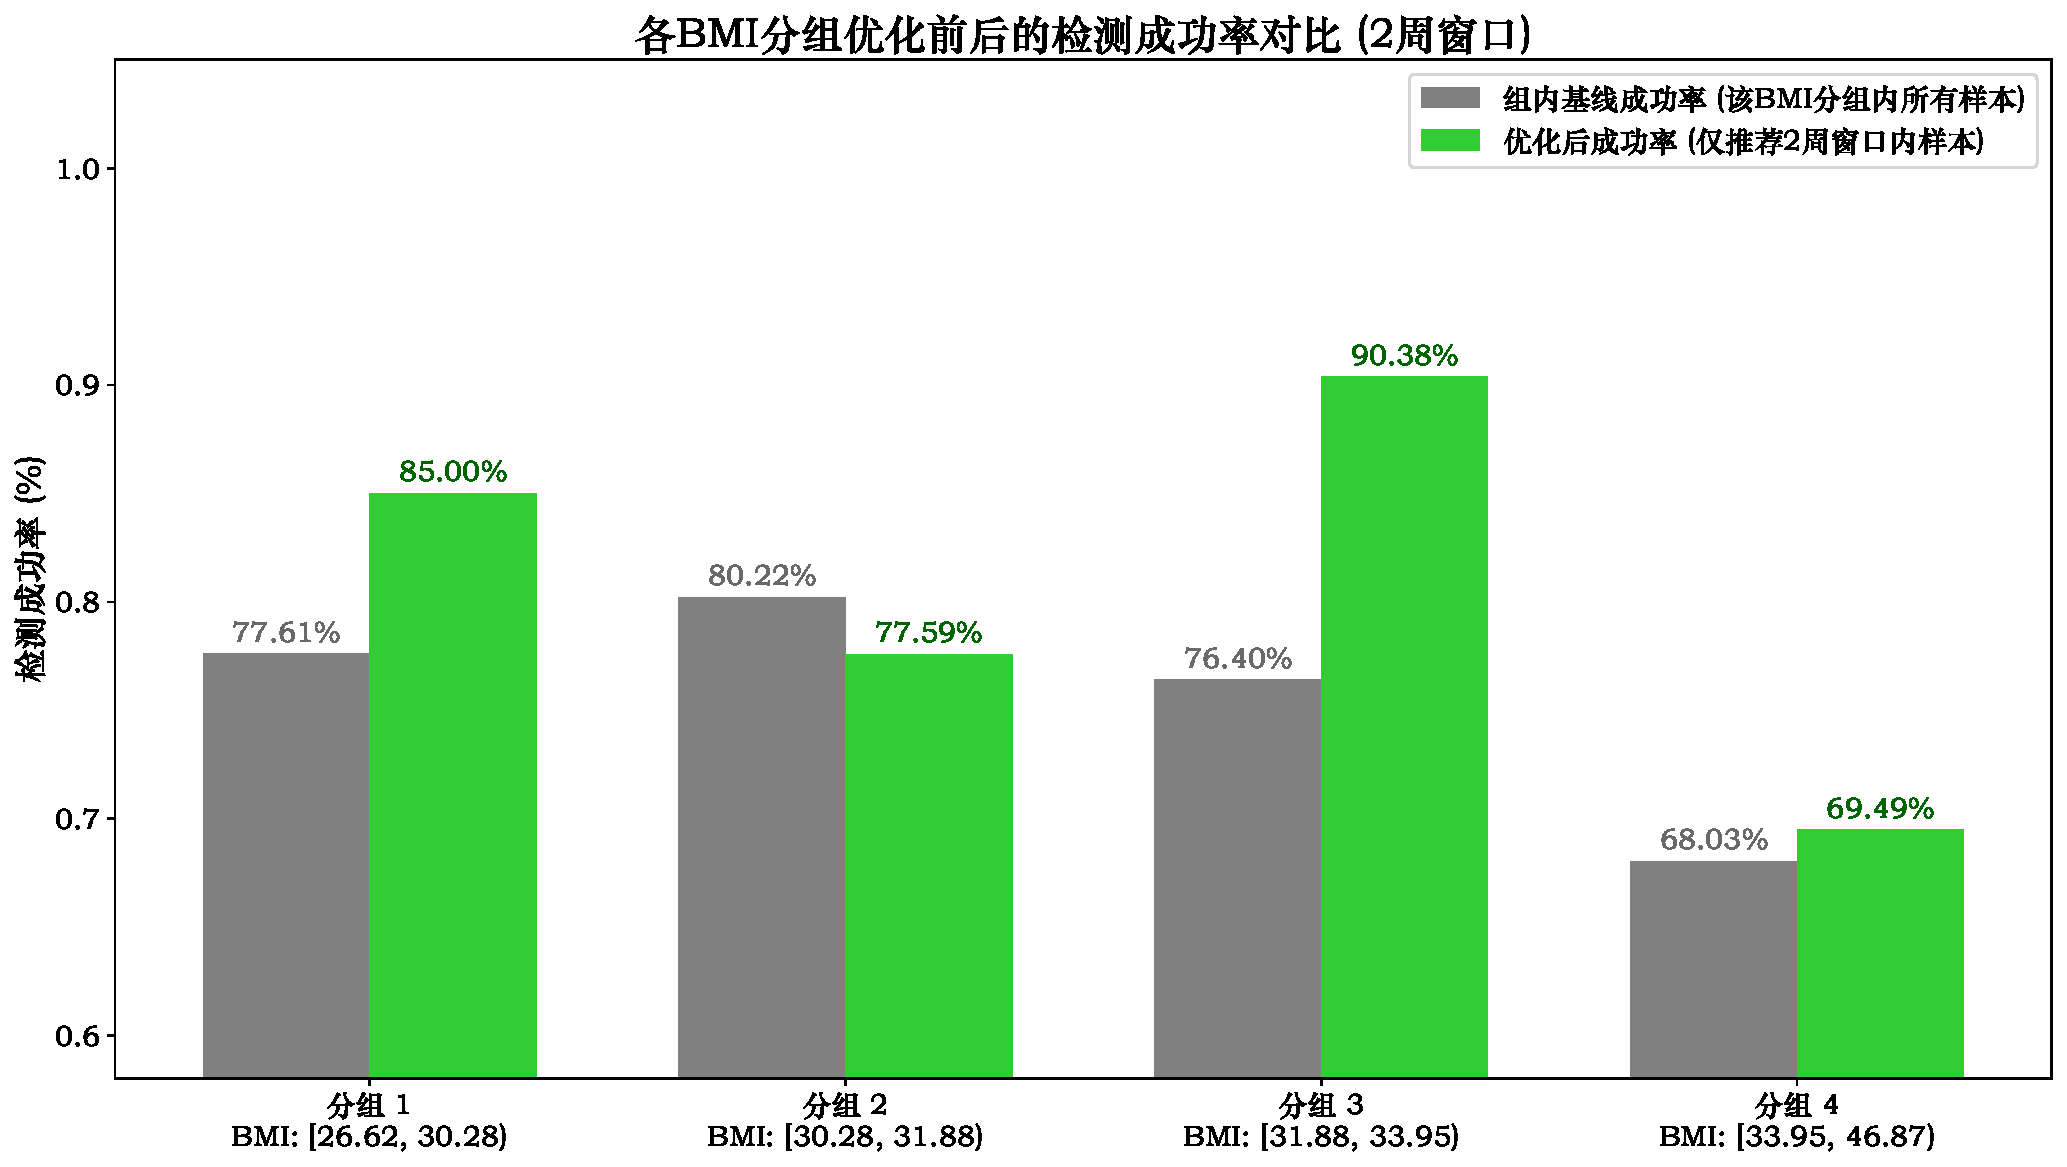
\includegraphics[width=0.8\textwidth]{chapters/Q2/images/组内检测成功率对比分析.pdf}
    \caption{组内检测成功率对比图}
    \label{fig:组内检测成功率对比图}
\end{figure}

对于分组1、3，本模型推荐的NIPT窗口极大地提升了检测成功率，而分组 2 略低于该组的基线水平的原因是模型为降低风险，选择了成功率稍低的窗口，该决策很可能使分组 3 的检测成功率大幅提升。证明了检测误差是塑造最终决策结果的驱动之一。它不仅是模型需要规避的对象，更是迫使模型进行智能权衡的关键因素。


\section{问题三的模型建立与求解}

本文中的问题一，已通过查阅论文断定男胎 Y 染色体浓度与年龄无关。且本文已通过式 \ref{eq:final_model} 拟合出男胎 Y 染色体浓度与孕周、BMI 之间的关系，于问题二的基础上，本文继续综合考虑 BMI（由于共线性，不考虑将体重与身高纳入模型）、检测误差、胎儿的 Y 染色体浓度达标比例等因素，新增了多个约束条件。

\subsection{数据预分析}

该图展示了在不同Y染色体浓度区间内，检测结果为“准确”的样本所占的比例。为保证统计稳健性，图中仅包含样本数大于$10$的区间。从图中可以清晰地观察到：当浓度低于$4\%$时，检测准确率显著下降；而当浓度高于$4\%$后，准确样本的比例提升并维持在较高水平。

为探究检测误差与Y染色体浓度的内在联系，并为优化模型构建更稳健的约束条件，本文绘制了准确样本比例随Y染色体浓度变化的分布图（如图 \ref{fig:Y染色体浓度与预测准确的关系} 所示）。

\begin{figure} [H]
    \centering
    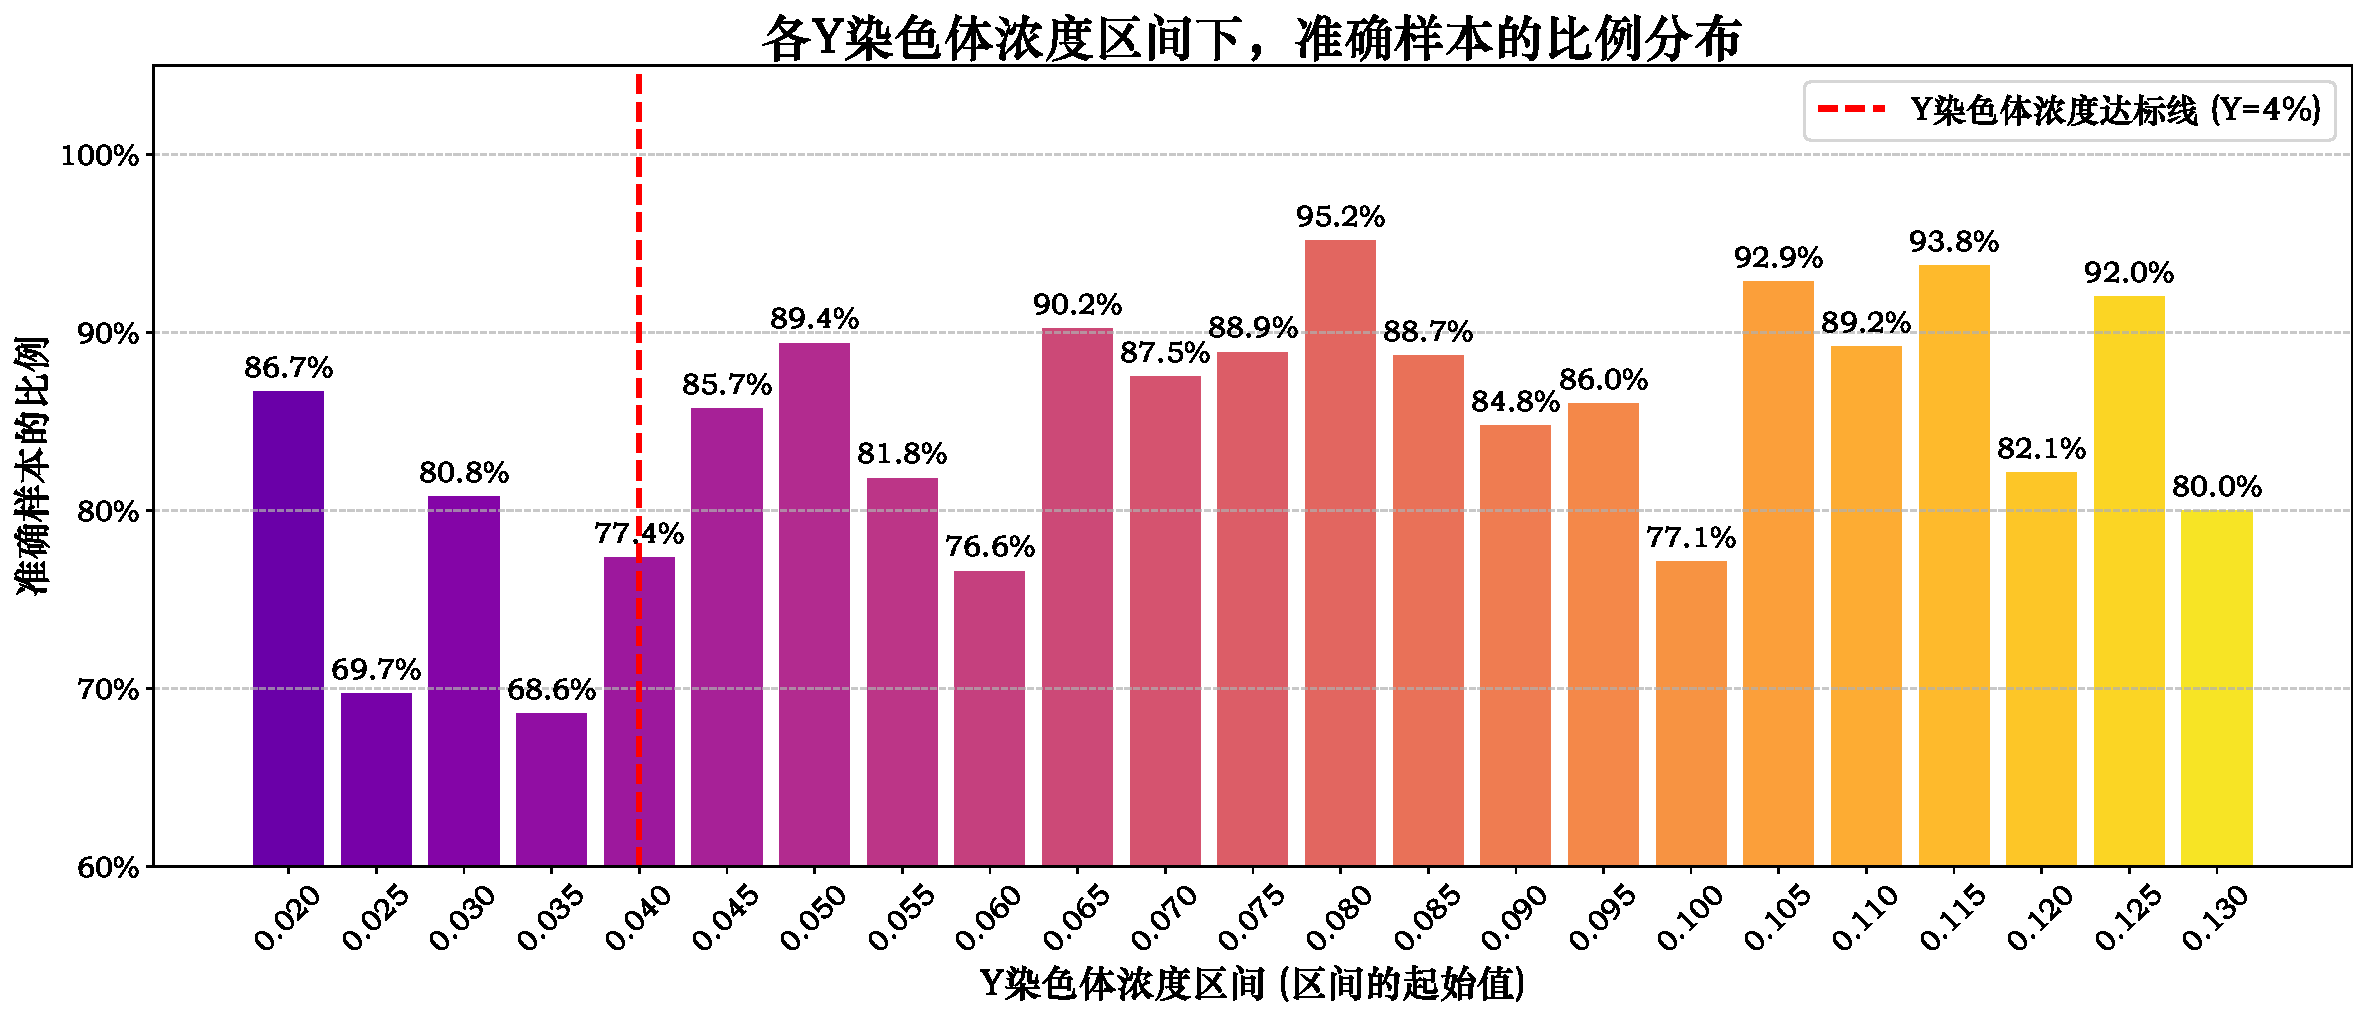
\includegraphics[width=0.8\textwidth]{chapters/Q3/images/Y染色体浓度与预测准确的关系.pdf}
    \caption{Y 染色体浓度与预测准确的关系}
    \label{fig:Y染色体浓度与预测准确的关系}
\end{figure}

\subsection{符号说明}

\begin{center}
    \begin{tabularx}{0.8\textwidth}{c@{\hspace{1pc}}|@{\hspace{2pc}}>{\centering\arraybackslash}X}
        \Xhline{0.08em} % 表格顶部粗线
        \textbf{符号}              & \textbf{符号说明（其余符号沿用上文符号）}               \\
        \Xhline{0.05em}
        $G_j$                    & 由边界点 $b_j$ 和 $b_{j+1}$ 定义的第 $j$ 个BMI分组。 \\
        $\hat{Y}(w, \text{bmi})$ & 根据第一问模型预测的Y染色体浓度。                       \\
        $P_{Y>6\%}(S_{j,w})$     & 窗口 $S_{j,w}$ 内Y染色体浓度大于6\%的样本比例。         \\
        \Xhline{0.08em}
    \end{tabularx}
\end{center}

\subsection{建立优化问题}

\subsubsection{目标函数}

此处，目标函数与问题二保持一致，参考式 \ref{eq:objective_function_final}.

\subsubsection{核心约束}

在$4\% \sim 6\%$的浓度区间内，准确率仍存在小幅波动，考虑到本文在问题一中所建立的预测模型 (\(Y = f(w, \text{BMI}, c)\)) 预测的是 Y 染色体浓度的数学期望，而任何临床单次测量的真实值都会围绕该均值存在随机波动。为规避随机波动的风险，且
基于图 \ref{fig:Y染色体浓度与预测准确的关系} 的数据，当Y染色体浓度超过$6\%$后，检测准确样本的比例更大。因此，本文构建如下约束条件，要求模型为各 BMI 分组推荐的最佳 NIPT 时点预测的 Y 染色体浓度理论值不低于$6\%$。
\begin{equation}
    \text{Y}_{ij} = f(w_{ij}^*, \text{BMI}_{ij}, c=1) \ge 0.06 \quad \forall j \in \{1, 2, 3, 4\}
    \label{eq:constraint_y_gt_6_percent}
\end{equation}
其中 $Y_{ij}$ 是第 $j$ 个分组中的第 $i$ 个孕妇在最佳孕周 $w_{ij}^*$ 时点的预测 Y 染色体浓度。

\subsubsection{软约束}

如果对于某个分组 $G_j$，在所有可能的孕周中都找不到任何一个能同时满足上述4个严格逻辑约束的窗口，模型会进入“宽松搜索”模式，只要求满足\textbf{窗口样本量约束}。然而，此时目标函数中的\textbf{惩罚项 $P(B)$}会被触发，其值会显著增大。这是一种软约束机制，它允许算法在找不到完美解时给出一个次优解，但会通过高昂的“罚分”来表明该解的质量有所欠缺，并激励算法继续寻找能满足所有严格约束的更优解。

\subsubsection{硬约束}

这些约束在优化过程中必须被严格满足。

\begin{enumerate}
    \item \textbf{边界点取值范围}: 所有BMI边界点 $b_i$ 必须位于数据集中BMI的最小值和最大值之间。
          \begin{equation}
              BMI_{\min} \le b_i \le BMI_{\max}, \quad \forall i \in \{1, \dots, 5\}
          \end{equation}

    \item \textbf{BMI分组最小宽度}: 为了避免产生过于狭窄、失去统计意义的分组，任意相邻两个边界点之间的差值必须不小于2.5。
          \begin{equation}
              |b_{i+1} - b_i| \ge 2.5, \quad \forall i \in \{1, \dots, 4\}
          \end{equation}
\end{enumerate}

\subsubsection{逻辑约束}

在目标函数内部，为每个给定的BMI分组 $G_j$ 寻找最佳孕周 $w_j^*$ 时，采用一个“严格-宽松”两阶段搜索策略。一个孕周窗口 $w_j$ 不仅要满足问题一的窗口长度，还必须满足以下\textbf{严格约束}，才被认为是理想的候选窗口：
\begin{enumerate}
    \item \textbf{窗口样本量}: 窗口内的样本数量 $N_{j,w}$ 必须在设定的范围内，以保证统计可靠性。
          \begin{equation}
              20 \le N_{j,w} \le 100
          \end{equation}
    \item \textbf{高Y浓度样本比例}: 窗口内，Y染色体浓度大于6\%的样本占比必须超过50\%，以确保窗口内的样本质量。
          \begin{equation}
              P_{Y>6\%}(S_{j,w}) \ge 0.50
          \end{equation}
\end{enumerate}

\subsection{差分进化求解}

本模型采用\textbf{差分进化}算法进行求解。差分算法是一种智能的启发式随机搜索算法，属于遗传算法的一种。它通过模拟生物进化过程中的变异、交叉和选择操作，在解空间中进行全局搜索。本文目标函数 $F(B)$ 依赖于对数据子集的复杂查询和搜索，且形态复杂（存在多个局部最优解）。对于这类问题，传统的梯度下降法难以奏效，而这样的全局优化算法则表现出色，能有效避免陷入局部最优，具有更强的鲁棒性。

我们通过调用 \texttt{scipy.optimize.differential\_evolution} 库函数来实现该算法。代码中设置了合理的种群大小（$popsize=30$）和最大迭代次数（$maxiter=100$），并启用了并行计算（$workers=4$）以加速收敛过程。经过差分进化算法优化求解，模型得到的最优BMI分组方案及对应的最佳 NIPT 时点建议如表 \ref{tab:q3_results} 所示。

\begin{table}[H]
    \centering
    \caption{最优BMI分组及NIPT时点推荐方案}
    \label{tab:q3_results}
    \begin{tabular}{cccc}
        \toprule
        \textbf{BMI分组} & \textbf{BMI区间} & \textbf{最佳NIPT时点 (周)} & \textbf{窗口内成功率} \\
        \midrule
        分组 1           & [29.07, 31.57) & 10 -- 12              & 80.00\%         \\
        分组 2           & [31.57, 34.11) & 11 -- 13              & 76.27\%         \\
        分组 3           & [34.11, 36.84) & 12 -- 14              & 77.78\%         \\
        分组 4           & [36.84, 43.07) & 23 -- 25              & 75.00\%         \\
        \bottomrule
    \end{tabular}
\end{table}

\v{-1em}

为直观验证该优化方案的有效性，本文将表 \ref{tab:q3_results} 中得到的四个最优NIPT推荐窗口，同样高亮矩形区域的形式叠加绘制在原始的散点图上，结果如图 \ref{fig:Q3_BMI分组和最佳NIPT时点} 所示 。从图中可以清晰地看出，模型推荐的窗口精确地覆盖了正常样本（蓝色点）的密集区域，同时有效规避了不准确样本（红色）和Y染色体浓度低于4\%的样本（橙色）的集中分布区。这直观地证实了模型在寻找最佳检测时点上的有效性。特别值得注意的是，对于BMI值最高的分组$4$（$BMI > 36.84$），模型推荐了一个明显更晚的检测窗口（$23 \sim 25$周），这与BMI越高、所需孕周越长的理论分析相符，进一步验证了模型的合理性。

\begin{figure}[H]
    \centering
    
\includegraphics[width=0.75\textwidth]{chapters/Q3/images/BMI分组和最佳NIPT时点.pdf}
    \caption{BMI分组和最佳NIPT时点}
    \label{fig:Q3_BMI分组和最佳NIPT时点}
\end{figure}

为进一步从数据层面评估本模型在规避检测误差方面的效果，本文采用了组内对比分析方法，将每个BMI分组在“推荐窗口”内的检测成功率与该组全体样本的“基线成功率”进行比较，对比结果如图 \ref{fig:Q3_组内检测成功率对比分析} 所示。

\begin{figure}[H]
    \centering
    
\includegraphics[width=0.8\textwidth]{chapters/Q3/images/组内检测成功率对比分析.pdf}
    \caption{组内检测成功率对比分析}
    \label{fig:Q3_组内检测成功率对比分析}
\end{figure}

\begin{itemize}
    \item 对于BMI较高的分组 $3$ 和分组 $4$，本模型计算所得的 NIPT 窗口极大地提升了检测成功率。分组 $3$ 的成功率从基线 $69.27\%$ 提升至 $77.78\%$ ，分组 $4$ 的成功率更是从 $60.29\%$ 大幅提升至 $75.00\%$。这表明对于高BMI这一高风险群体，本模型能有效定位到可显著降低检测失败风险的“黄金窗口”。
    \item 对于分组 $1$ 和分组 $2$，推荐窗口的成功率与基线水平相当（分组 $1$：$80.00\%$ VS $80.46\%$；分组 $2$：$76.27\%$ VS $76.97\%$）。这并非模型失效，而是多目标优化的必然结果。对于中低BMI的孕妇，可选的优质检测窗口较多，模型在保证高成功率的同时，会倾向于选择孕周更早的窗口以降低潜在风险。
\end{itemize}

综上所述，无论是从最优窗口的可视化定位，还是从组内成功率的量化对比来看，本文构建的模型及其求解结果都表现出良好的有效性和稳健性。它不仅能为不同BMI水平的孕妇群体提供定制化的 NIPT 时点建议，更能通过智能权衡，显著提升高风险群体的检测成功率，从而有效规避检测误差。

\section{问题四的模型建立与求解}

\subsection{方法的选择与数据预分析}

考虑到此问题的要求是综合考虑各项指标，得到一个对异常女胎的判断方法，本文决定构建基于机器学习的分类模型。本文选择使用机器学习方法进行求解。数据方面，若孕妇的染色体的非整倍体出现T13、T18、T21中任一异常，那么本文将其标记为“异常女胎”，否则标记为“正常女胎”。同时注意到当妊娠方式为试管婴儿时，仅有 $1$ 个样本出现了染色体非整倍体，样本不足以支撑模型的建立，因此本文不将妊娠方式考虑在因素内。

统计发现，女胎数据染色体的非整倍体分布中，胎儿患 T18 与 T13 的比重相近，T21 的比重较大，约为 T18、T13 的四倍。

\begin{figure} [H]
    \centering
    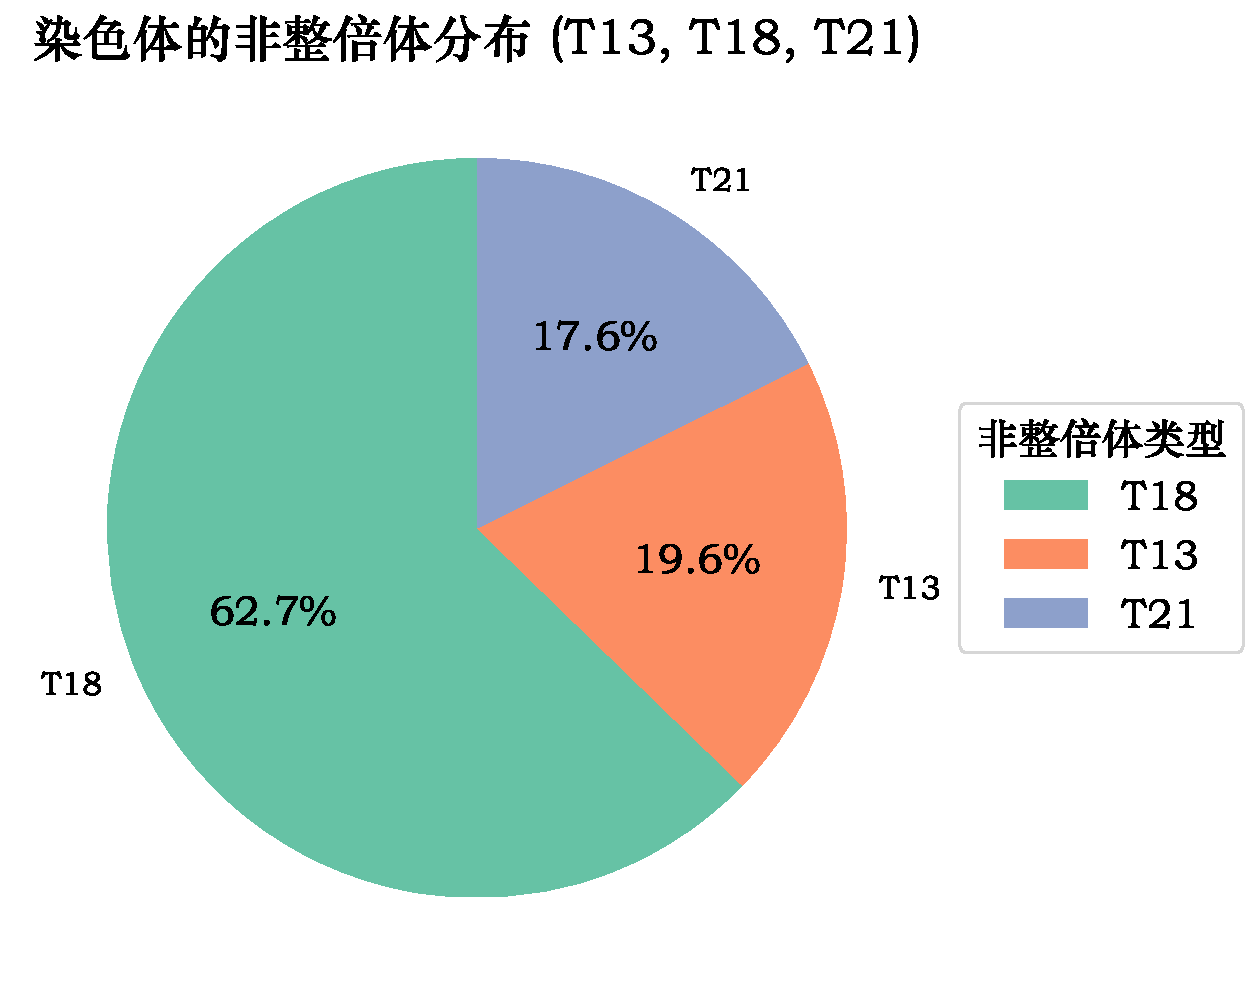
\includegraphics[width=0.4\textwidth]{chapters/Q4/images/非整倍体扇形图.pdf}
    \caption{非整倍体扇形图}
    \label{fig:非整倍体扇形图}
\end{figure}

为了直观地探索各个特征对女胎异常的区分能力，本文采用核密度估计绘制每个特征的平滑概率分布图。通过在同一图表上叠加对比正常样本与异常样本的分布（图 \ref{fig:核心指标对比图}，其余非核心指标见附录图 \ref{fig:其他指标对比图}），发现绝大多数特征的分布曲线都高度重合，而仅在13号、18号、21号及 X 染色体的浓度这几个关键指标上，异常样本的分布曲线显著地向高分区域偏移，可合理猜测X染色体浓度是用于判定女胎异常的最显著特征。

\begin{figure} [H]
    \centering
    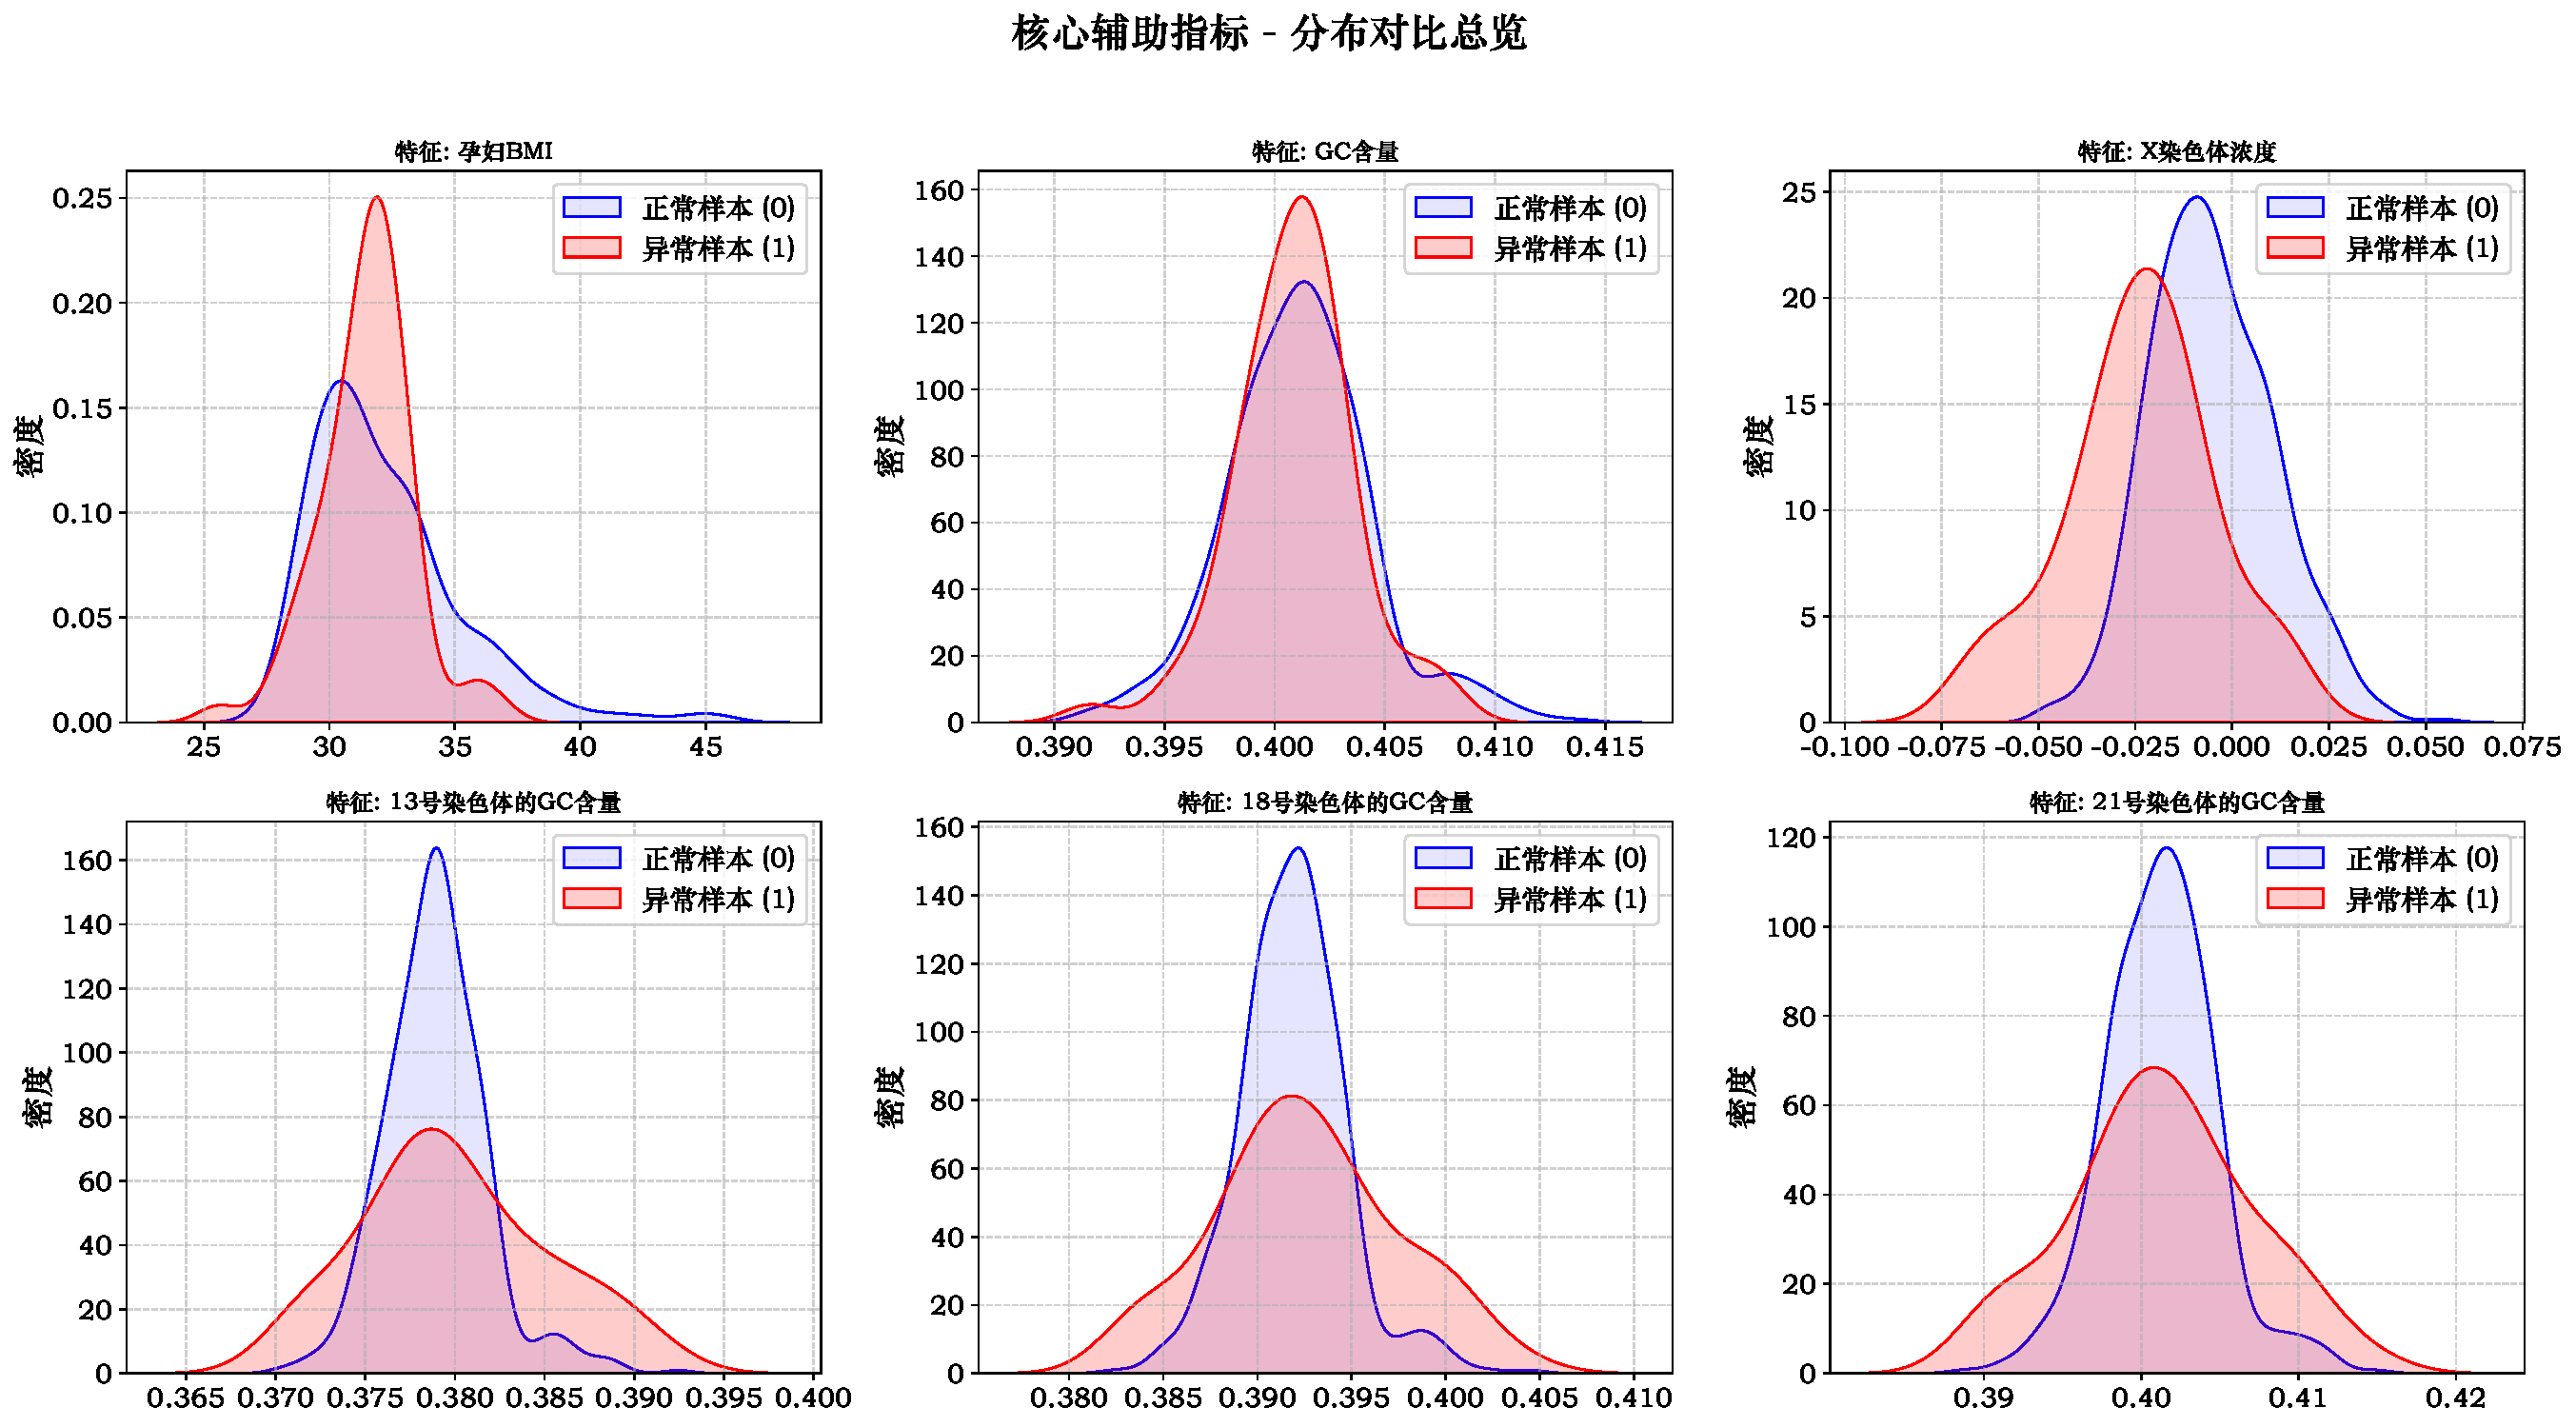
\includegraphics[width=0.9\textwidth]{chapters/Q4/images/核心指标对比图.pdf}
    \caption{核心指标对比图}
    \label{fig:核心指标对比图}
\end{figure}

\subsection{模型优化}

XGBoost是一种高效的梯度提升算法，它的革新主要体现在其对目标函数的重新定义和高效的求解策略上，同时显著提升了训练速度和模型性能。具体来说，XGBoost通过其独特的提升机制，能够捕捉到预测变量之间复杂的、非线性的相互作用关系。在本题中，胎儿是否异常可能并非由单一指标决定，而是多个因素共同作用的结果，而该模型强大的模式识别能力使其能够精确地学习这些复杂的决策边界。在第 $t$ 轮迭代中，XGBoost 需要优化的目标函数由两部分组成，训练损失和正则化项。训练损失和正则化项的定义如下：
\begin{equation}
    \text{Obj}^{(t)} = \sum_{i=1}^{n} l\left(R_i, \hat{y}_i^{(t)}\right) + \sum_{k=1}^{t} \Omega(f_k)  \qquad     \Omega(f_t) = \gamma T + \frac{1}{2}\lambda \sum_{j=1}^{T} w_j^2
\end{equation}
其中，$n$ 是样本总数， $R_i$ 是第 $i$ 个样本“染色体的非整倍体”的真实检测结果，$l(\cdot)$ 是损失函数，用于衡量真实值 $R_i$ 与预测值 $\hat{y}_i^{(t)}$ 之间的差异，$\Omega(f_k)$ 是第 $k$ 棵树的正则化项，$T$ 是树 $f_t$ 的叶子节点数量，$w_j$ 是第 $j$ 个叶子节点的权重（即分数），$\gamma$ 和 $\lambda$ 是控制复杂度的超参数。

注意到附件中异常女胎样本远少于正常样本，直接使用标准XGBoost模型可能会导致对异常胎儿的识别能力不足。当某一类别的样本数量占据绝对优势时，模型会发现将所有样本都预测为多数类，便可以轻易获得非常高的准确率。这种现象导致模型对异常样本的识别能力极差。Zhang et al.在研究中指出，XGBoost算法在直接处理类别不平衡的数据时，其分类效果往往并不理想，可能会对少数类样本产生较高的误分类率\cite{zhang2022research}。因此我们需要对数据进行采样处理，将异常样本和正常样本的数量调整到相近水平。

\subsection{数据采样}

本文最初考虑采用随机上采样、随机下采样方法来使异常女胎的个数与正常女胎的个数相当。随机上采样是随机复制少数类样本，使正负样本数量达到平衡；随机下采样是随机丢弃多数类样本以实现平衡。然而在实际应用中，本文发现随机上采样和随机下采样的效果并不理想。由于异常样本过少，随机上采样会对少数类进行过多的复制，导致模型过拟合，虽然准确率高，但本文发现其对异常样本的识别能力并不强；基于同样的原因，随机下采样可能丢失多数类的重要信息，导致模型的识别能力不足，因此查阅相关文献后，本文决定选用SMOTE\cite{DeepSeek_2}对数据进行处理。

SMOTE的核心思想并非简单地复制少数类实例，而是通过在特定邻域内的几个少数类实例之间进行插值而创建数据点。该算法的计算基于数据的特征值及其关系，而不是将数据点作为一个整体来考虑\cite{fernandez2018smote}。但是SMOTE的短板在于过度泛化，在创建数据的时候可能也会产生噪声数据，因其无法区分不同类别。而Tomeklink是去除多数类中噪声数据的一种方法，可以清除具有相似特征和重叠的多数类中的噪声数据。但作为欠采样方法，Tomeklink移除的样本数量有限，对于严重不平衡的数据集，其改善效果可能不足在实际实现中。Tomeklink和SMOTE过采样结合起来，比单独使用两种方法的效果更好\cite{hairani2023improvement}，因此本文采用这种方法对数据进行采样。

\subsection{模型建立与求解}
本文使用Python的XGBoost库来实现XGBoost分类模型。首先将数据集划分为训练集和测试集，其中，测试集在整个模型训练和优化过程中保持不可见，仅用于最终评估模型的性能。为确保划分后的训练集和测试集中异常样本的比例与原始数据一致，本文采用了\textbf{分层抽样}的方法。随后，将前述的\textbf{SMOTETomek方法}应用于训练集，生成一个类别均衡的、用于模型训练的新数据集。测试集则保持其原本的样本分布，以模拟模型在真实世界数据上的表现，训练流程图如图 \ref{fig:训练流程图} 所示。

\begin{figure}[H]
    \centering
    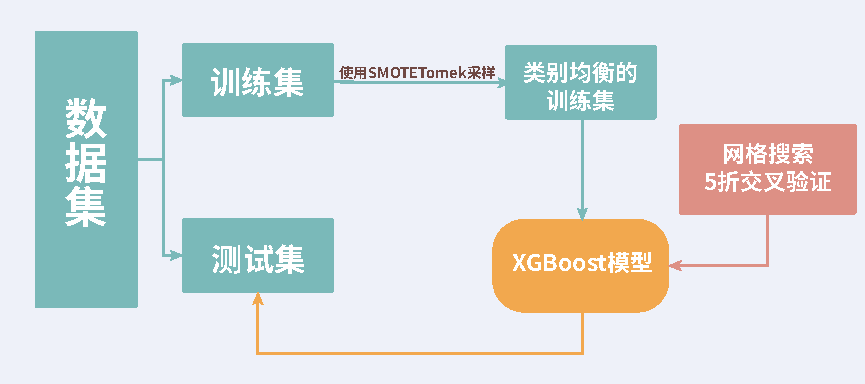
\includegraphics[width=0.5\textwidth]{chapters/Q4/images/xgboost训练流程.pdf}
    \caption{训练流程图}
    \label{fig:训练流程图}
\end{figure}

为了寻找到XGBoost模型的最佳性能，本文将网格搜索与5折交叉验证相结合对模型的关键超参数进行寻优。考虑到在临床诊断中，将异常胎儿误判为正常（即\textbf{漏报，假阴性}）带来的后果是巨大的，而误将正常胎儿误判为异常（即\textbf{误报，假阳性}）的代价相对可控\cite{odibo2005cost}，漏报比误报的代价更大，因此本文选择召回率(Recall)作为网格搜索过程中的核心评估指标。在找到最优超参数组合后，将模型经过在SMOTETomek采样处理后的完整训练集上训练，得到最终的XGBoost分类模型，性能评估报告如图 \ref{tab:performance_report} 所示，数据情况与模型混淆矩阵如图 \ref{fig:数据情况与模型表现情况图} 所示：
\begin{figure}[H]
    \centering
    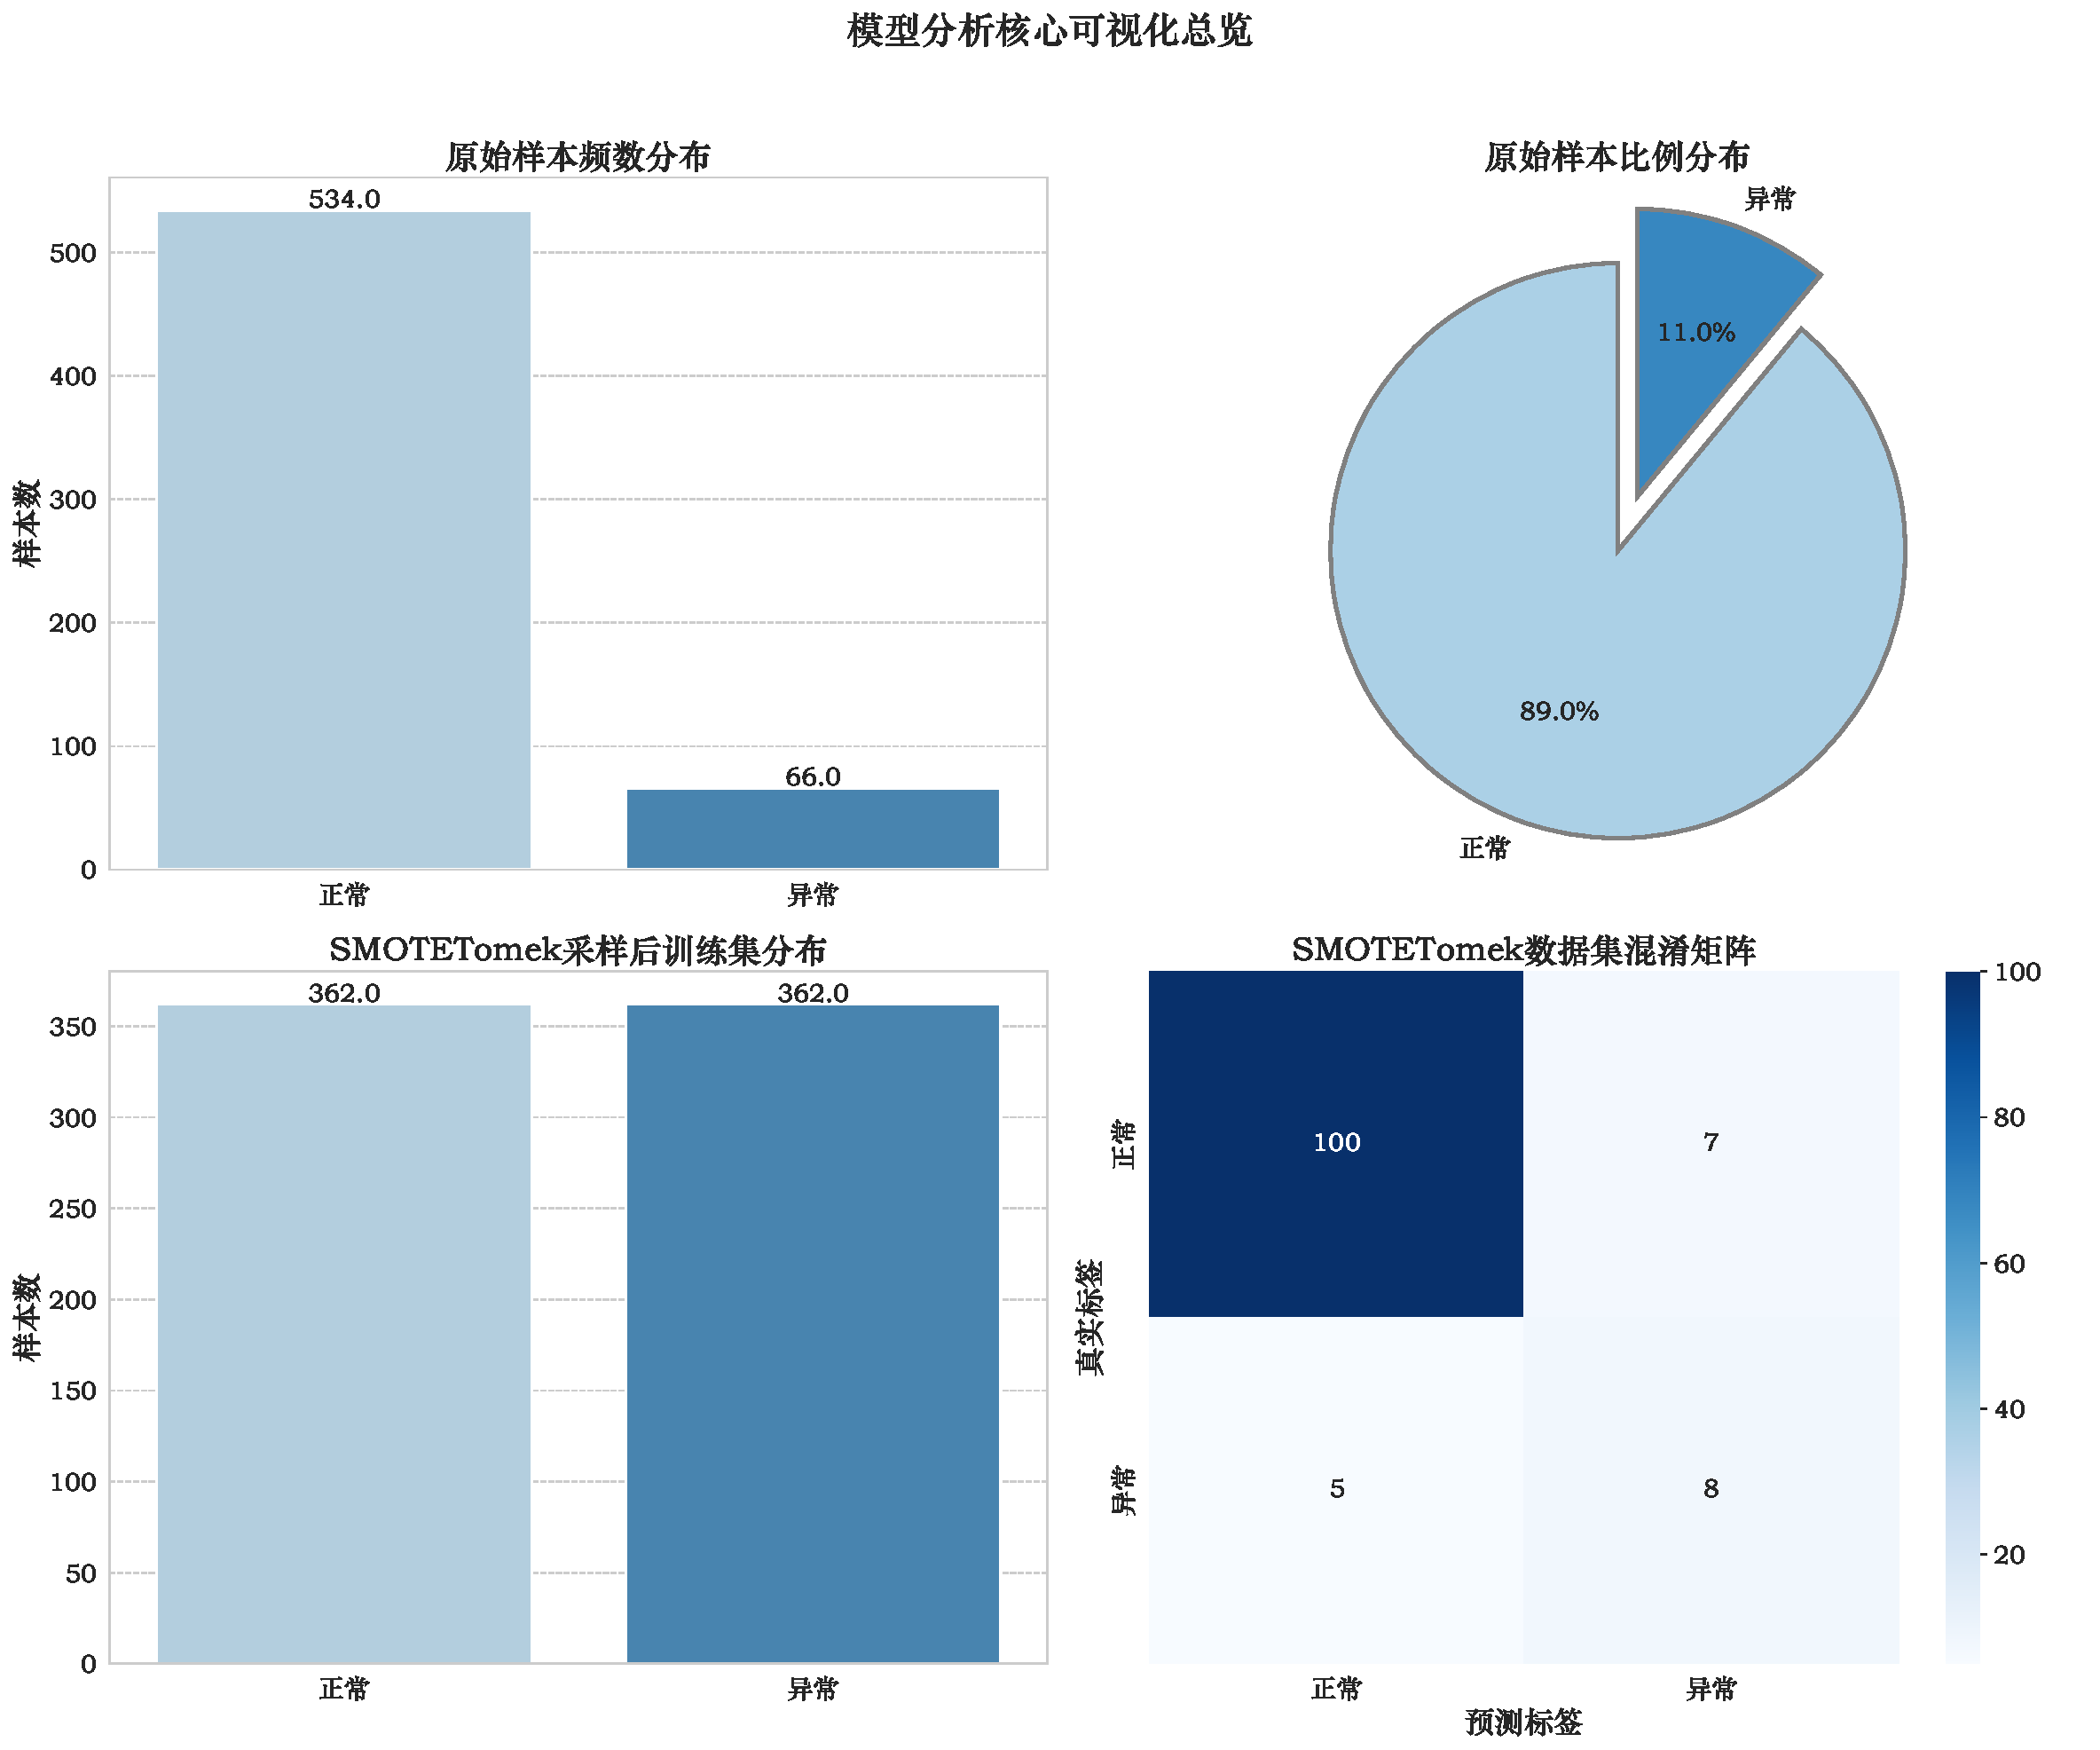
\includegraphics[width=0.65\textwidth]{chapters/Q4/images/核心可视化总览.pdf}
    \caption{数据情况与模型表现情况图}
    \label{fig:数据情况与模型表现情况图}
\end{figure}

\begin{table}[H]
    \centering
    \caption{分类模型性能评估报告}
    \label{tab:performance_report}
    \begin{tabular}{lcccc}
        \toprule
        \textbf{}             & \textbf{Precision} & \textbf{Recall} & \textbf{F1-score} & \textbf{Support} \\
        \midrule
        \textbf{类别 0}         & 0.95               & 0.93            & 0.94              & 107              \\
        \textbf{类别 1}         & 0.53               & 0.62            & 0.57              & 13               \\
        \midrule
        \textbf{accuracy}     &                    &                 & 0.90              & 120              \\
        \textbf{macro avg}    & 0.74               & 0.77            & 0.76              & 120              \\
        \textbf{weighted avg} & 0.91               & 0.90            & 0.90              & 120              \\
        \bottomrule
    \end{tabular}
\end{table}

同时我们也进行了特征的重要性分析，结果如图 \ref{fig:特征重要性} 所示。可以看出，X染色体浓度的特征重要性最高，这与我们前面通过核密度估计所观察到的结果是一致的。

\begin{figure} [H]
    \centering
    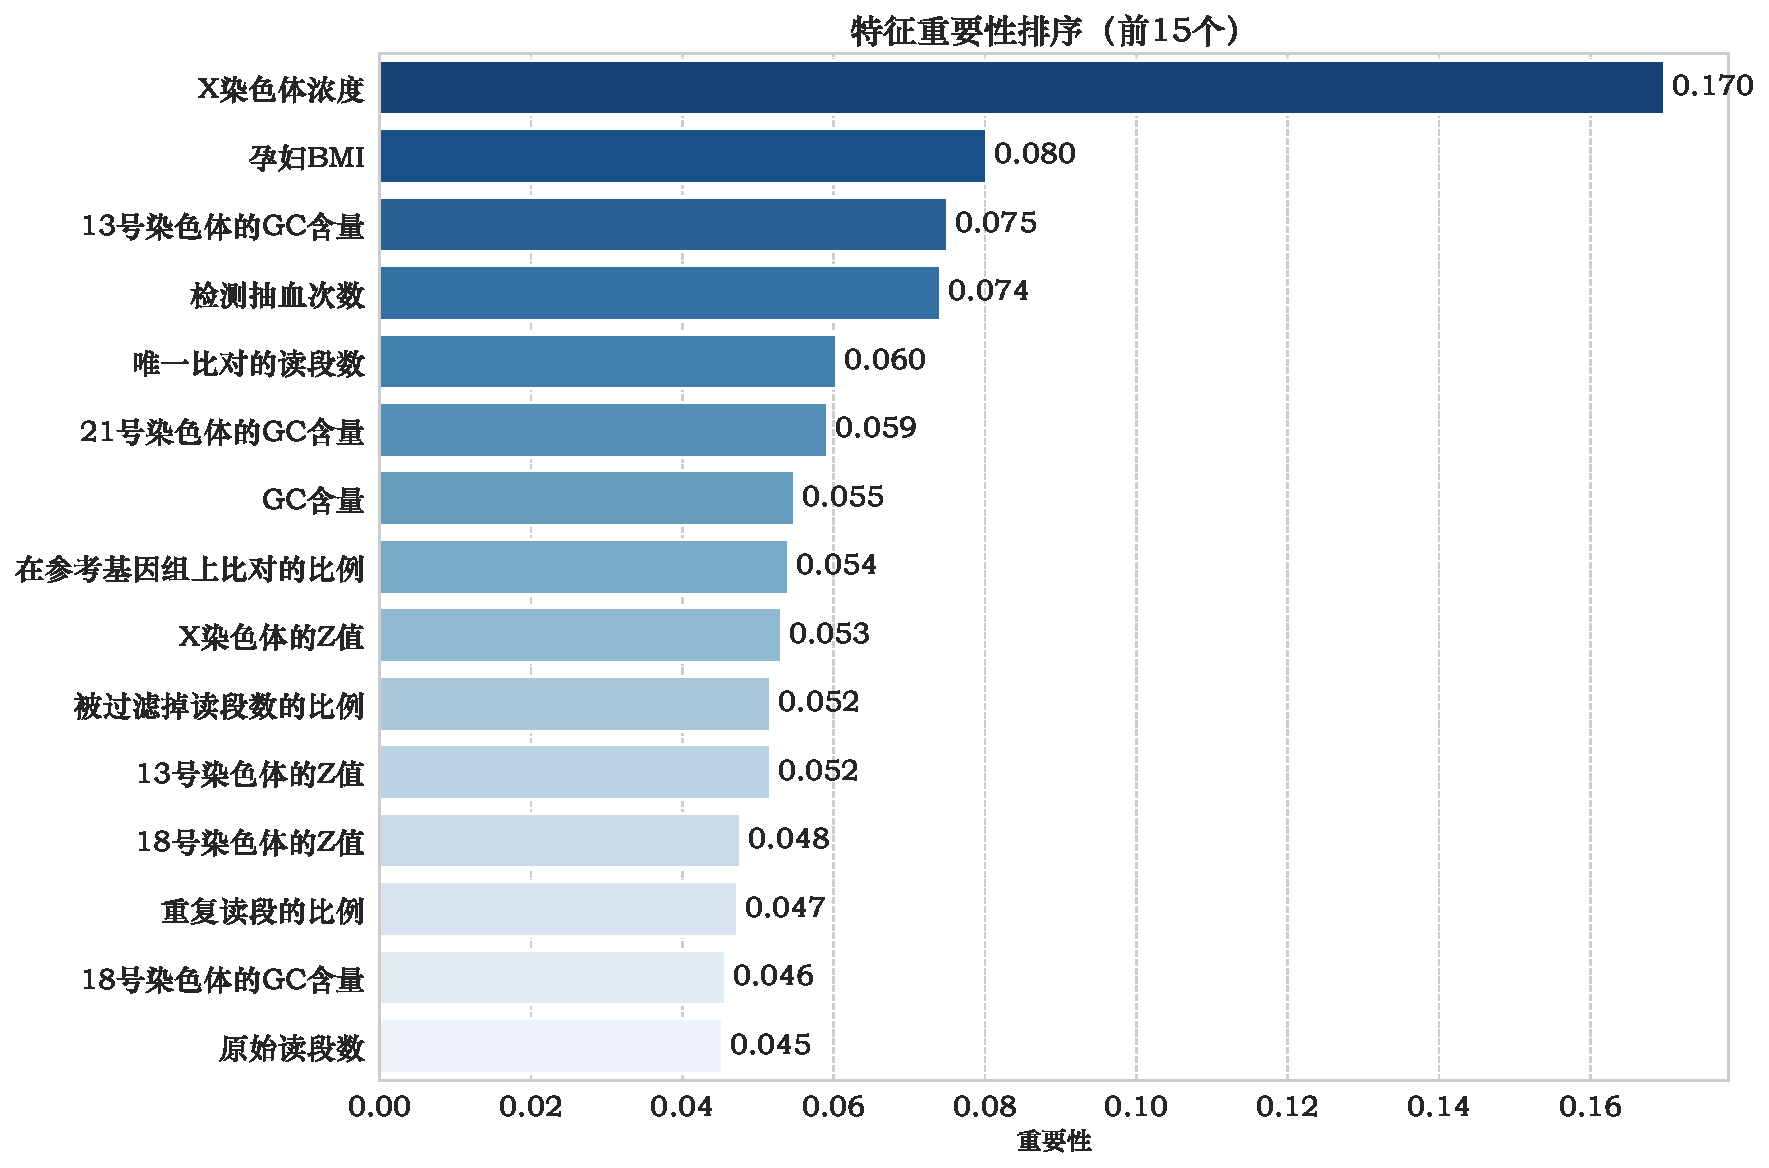
\includegraphics[width=0.7\textwidth]{chapters/Q4/images/特征重要性.pdf}
    \caption{特征重要性}
    \label{fig:特征重要性}
\end{figure}

\subsection{判定预测方法}


本文构建的XGBoost模型在完成预测后，并不会直接输出“异常”或“正常”的二元标签，而是给出一个介于 $[0, 1]$ 之间的连续概率值。该概率值代表了模型预测某个样本为“异常”的可信度。因此，我们需要设定一个\textbf{决策阈值}，当模型输出的概率大于等于该阈值时，则将样本判定为“异常”，反之则为“正常”。因此，选择一个科学、合理的决策阈值，是本判定方法能够应用于实践的关键一步。

为了找到能够最好地平衡“不漏诊”和“不误诊”这对矛盾需求的阈值，本文选择寻找F1值最高值对应的概率值。而要计算F1，也需要\textbf{精确率}和\textbf{召回率}这两个核心评估指标。

\textbf{精确率}是所有被预测为“异常”的样本中，真异常样本的比例，即：
\begin{equation}
    \text{Precision} = \frac{\text{TP}}{\text{TP} + \text{FP}}
    \label{eq:precision}
\end{equation}
其中TP是真正例，FP是假正例。高精确率意味着模型的预测结果误报率低。

\textbf{召回率}是所有真正是“异常”的样本中，被模型成功预测出来的比例。即：
\begin{equation}
    \text{Recall} = \frac{\text{TP}}{\text{TP} + \text{FN}}
    \label{eq:recall}
\end{equation}
其中FN是假反例。高召回率意味着模型的漏报率低。

\textbf{F1分数}是精确率和召回率的调和平均数，是同时考虑这两个指标的综合性评价指标。其计算公式为：
\begin{equation}
    F_1 = 2 \cdot \frac{\text{Precision} \cdot \text{Recall}}{\text{Precision} + \text{Recall}}
    \label{eq:f1_score}
\end{equation}

只有当精确率和召回率二者都较高时，F1分数才会高，因此选择F1分数最高值即能得到在“误判”和“漏判”两方面兼顾的最佳阈值。

本文的最优阈值判定方法为遍历所有可能的决策阈值，计算出在每一个阈值下模型在测试集上的精确率和召回率，并由此得到对应的F1分数。最终选取能够使\textbf{F1分数达到最大值}的那个阈值作为最终的判定标准，计算过程如图 \ref{fig:阈值选择} 所示。经过计算，本文得到的最优决策阈值为 $0.8128$，对应的最高F1分数是$0.571$。

\begin{figure}[H]
    \centering
    
\includegraphics[width=0.8\textwidth]{chapters/Q4/images/阈值选择可视化.pdf}
    \caption{阈值选择}
    \label{fig:阈值选择}
\end{figure}

为了能够通过给定单条数据判定女胎是否异常，本文能够提供基于训练好的分类模型的预测交互。在模型训练代码中，训练结束后可允许用户输入 $16$ 个关键特征参数，模型将基于这些输入数据计算并输出胎儿异常的风险概率。模型输出两个概率值：正常概率和异常概率，异常概率即为胎儿存在染色体非整倍体异常的风险评估值，该数值介于 $0 \sim 1$ 之间，若异常概率大于上文所计算出的最优决策阈值 $0.8128$，则判定为“异常”，否则判定为“正常”。

\section{优缺点分析}

\subsection{优点分析}
\begin{enumerate}
    \item \textbf{数据处理的科学性与严谨性}：在问题一中，通过计算ICC识别并采用混合效应模型处理重复测量数据，避免了传统回归的统计谬误。在问题四中，本文敏锐地捕捉到严重的类别不平衡问题，并选用了先进的SMOTE-Tomek混合采样技术，有效避免了模型偏向多数类，为后续精准分类奠定基础。

    \item \textbf{建模思路的递进性与关联性}：四个问题并非孤立解决，而是形成了一个有机的整体。问题一建立的Y染色体浓度预测模型 $Y = f(w, \text{BMI}, c)$，在问题三中被巧妙地用作核心约束条件，确保了推荐时点的理论可靠性。这种模型之间的调用与联动，体现了本文系统性解决问题的能力。

    \item \textbf{优化目标的临床实际导向}：在问题二和问题三的优化模型中，本文没有仅仅追求单一目标，而是构建了平衡“降低潜在风险”与“提升检测成功率”的多目标优化框架。特别是在权重设置和超参数寻优时，本文始终将临床后果（如漏诊风险大于误诊）作为优先考量，使得模型决策更贴近实际需求。
    \item \textbf{算法选择的先进性与匹配度}：本文根据不同问题的特性，选用了最合适的算法。例如，面对问题三中形态复杂、存在多个局部最优解的目标函数，本文采用鲁棒性更强的差分进化全局优化算法。在问题四中，选用了性能卓越的XGBoost分类器，并结合交叉验证与网格搜索进行精细调优，确保了模型的性能上限。
\end{enumerate}

\subsection{缺点分析}

\begin{enumerate}

    \item \textbf{对异常样本的依赖性}：在问题四的分类模型中，尽管本文使用了SMOTE-Tomek技术来扩充和清洗样本，但模型的训练效果本质上仍高度依赖于原始数据中有限的异常样本特征。如果原始异常样本的代表性不足或存在某种偏差，合成出的新样本也可能继承这些偏差，从而影响模型的泛化能力。

    \item \textbf{模型解释性的权衡}：本文选用的XGBoost 和差分进化 等算法虽然性能强大，但其内在决策逻辑比线性模型等传统方法更为复杂，属于“黑箱”或“灰箱”模型。虽然本文通过特征重要性等方法进行了事后分析，但在向临床医生解释“为何模型会做出如此具体的判断”时，其直观性和透明度相对较低。

    \item \textbf{检测窗口推荐的复杂性}：在问题二中，虽然 BMI 最高的组$[33.95, 46.87)$确实推荐了最晚的检测窗口（$23 \sim 24$周），但 BMI 在 $[31.88, 33.95)$ 区间的孕妇，其最优窗口（$13 \sim 14$周）反而早于前一区间。这表明，简单的趋势外推不足以确定最优检测时点，必须综合考虑特定 BMI 区间内样本的实际分布、检测成功率和潜在风险。

\end{enumerate}

\newpage

\printbibliography[heading=bibliography,title=参考文献]
% \bibliography{references}

\newpage

\begin{center}
    \Large\bfseries
    附录
\end{center}

\addappendix{支撑材料文件列表}

% Notice: 注意，支撑文件的文字请使用仿宋字体 \fangsong

% Q1 文件夹
\section*{Q1 文件夹文件列表}
\begin{table}[H]
    \centering
    \fangsong
    \begin{tabularx}{\textwidth}{>{\RaggedRight}X >{\RaggedRight}X}
        \toprule
        \textbf{文件名}          & \textbf{简介}      \\
        \midrule
        AIC和BIC检验.py          & AIC和BIC检验代码      \\
        Y染色体浓度与有关系的变量的散点图.pdf & Y染色体浓度与相关变量散点图   \\
        Y染色体浓度与自身变量散点图.py     & Y染色体浓度与自身变量散点图代码 \\
        四个自变量的散点图.pdf         & 四个自变量散点图         \\
        四个自变量的散点图.py          & 四个自变量散点图代码       \\
        多重共线性检测.py            & 多重共线性检测代码        \\
        非线性混合模型.py            & 非线性混合模型代码        \\
        预测值与真实值.pdf           & 预测值与真实值对比图       \\
        \bottomrule
    \end{tabularx}
\end{table}

% Q2 文件夹 - BMI分组
\section*{Q2 文件夹文件列表}
\subsection*{BMI分组}
\begin{table}[H]
    \centering
    \fangsong
    \begin{tabularx}{\textwidth}{>{\RaggedRight}X >{\RaggedRight}X}
        \toprule
        \textbf{文件名}   & \textbf{简介} \\
        \midrule
        BMI分组.py       & BMI分组代码     \\
        孕妇BMI的四分位点.pdf & 孕妇BMI四分位点分析 \\
        \bottomrule
    \end{tabularx}
\end{table}

% Q2 文件夹 - KMeans与加权和
\subsection*{KMeans与加权和}
\begin{table}[H]
    \centering
    \fangsong
    \begin{tabularx}{\textwidth}{>{\RaggedRight}X >{\RaggedRight}X}
        \toprule
        \textbf{文件名}       & \textbf{简介}       \\
        \midrule
        BMI分组和最佳NIPT时点.pdf & BMI分组与最佳NIPT时点关系图 \\
        BMI聚类分析结果.pdf      & BMI聚类分析结果图表       \\
        K-Means手法.pdf      & K-Means聚类方法介绍     \\
        KMeans对BMI聚类.py    & K-Means对BMI聚类代码   \\
        加权和法.py            & 加权和算法代码           \\
        加权和法与二周窗口优化.py     & 加权和法两周窗口优化代码      \\
        组内检测成功率对比分析.pdf    & 组内检测成功率对比图        \\
        \bottomrule
    \end{tabularx}
\end{table}

% Q2 文件夹 - 数据预处理
\subsection*{数据预处理}
\begin{table}[H]
    \centering
    \fangsong
    \begin{tabularx}{\textwidth}{>{\RaggedRight}X >{\RaggedRight}X}
        \toprule
        \textbf{文件名}            & \textbf{简介}        \\
        \midrule
        BMI与孕周散点图.pdf           & BMI与孕周关系散点图        \\
        BMI与孕周散点图.py            & BMI与孕周关系散点图代码      \\
        优化模型.py                 & 模型优化代码             \\
        剔除Y小于4的散点图.py           & 剔除Y值小于4的散点图代码      \\
        剔除Y小于4的散点图 (标注不正确点).pdf & 剔除Y值小于4并标注不正确点的散点图 \\
        标注全部不准确散点图.pdf          & 标注所有不准确点的散点图       \\
        标注全部不准确散点图.py           & 标注所有不准确点散点图代码      \\
        添加结果检验结果列.py            & 添加结果检验列代码          \\
        \bottomrule
    \end{tabularx}
\end{table}

% 数据预处理文件夹 (第二张图片)
\subsection*{数据预处理 (续)}
\begin{table}[H]
    \centering
    \fangsong
    \begin{tabularx}{\textwidth}{>{\RaggedRight}X >{\RaggedRight}X}
        \toprule
        \textbf{文件名}   & \textbf{简介}   \\
        \midrule
        GC值小提琴图.pdf    & GC值分布小提琴图     \\
        GC值小提琴图.py     & GC值小提琴图代码     \\
        孕天数是否正确.py     & 检查孕天数代码       \\
        孕妇检测次数直方图.py   & 孕妇检测次数直方图代码   \\
        年龄均值差异分析.py    & 年龄均值差异分析代码    \\
        检测BMI异常值.py    & 检测BMI异常值代码    \\
        检测孕周转为孕天.py    & 孕周转孕天代码       \\
        检测次数.pdf       & 检测次数图表        \\
        检测表格空值.py      & 检测表格空值代码      \\
        清洗女胎数据.py      & 清洗女胎数据代码      \\
        统一表格时间.py      & 统一表格时间格式代码    \\
        统计非大龄Y染色体均值.py & 统计非大龄Y染色体均值代码 \\
        \bottomrule
    \end{tabularx}
\end{table}

% Q3 文件夹
\section*{Q3 文件夹文件列表}
\begin{table}[H]
    \centering
    \fangsong
    \begin{tabularx}{\textwidth}{>{\RaggedRight}X >{\RaggedRight}X}
        \toprule
        \textbf{文件名}       & \textbf{简介}       \\
        \midrule
        BMI分组和最佳NIPT时点.pdf & BMI分组与最佳NIPT时点关系图 \\
        Y染色体浓度与预测准确的关系.pdf & Y染色体浓度与预测准确性关系图   \\
        Y染色体浓度与预测准确的关系.py  & Y染色体浓度与预测准确性关系图代码 \\
        差分算法.py            & 差分算法代码            \\
        组内检测成功率对比分析.pdf    & 组内检测成功率对比图        \\
        \bottomrule
    \end{tabularx}
\end{table}

% Q4 文件夹
\section*{Q4 文件夹文件列表}
\subsection*{GBDT}
\begin{table}[H]
    \centering
    \fangsong
    \begin{tabularx}{\textwidth}{>{\RaggedRight}X >{\RaggedRight}X}
        \toprule
        \textbf{文件名} & \textbf{简介} \\
        \midrule
        Q4\_solve.py & Q4问题求解代码    \\
        核心可视化总览.pdf  & 核心可视化总览图表   \\
        特征重要性.pdf    & 特征重要性分析图    \\
        阈值选择可视化.pdf  & 阈值选择可视化图    \\
        \bottomrule
    \end{tabularx}
\end{table}

% Q4 文件夹 - 数据分析
\subsection*{数据分析}
\begin{table}[H]
    \centering
    \fangsong
    \begin{tabularx}{\textwidth}{>{\RaggedRight}X >{\RaggedRight}X}
        \toprule
        \textbf{文件名}             & \textbf{简介}         \\
        \midrule
        不同特征在检验正确或错误样本中的分布对比.pdf & 不同特征在正确/错误样本中的分布对比图 \\
        其他指标对比图.pdf              & 其他指标对比图             \\
        异常样本分布.py                & 异常样本分布分析代码          \\
        数据分布分析.py                & 数据分布分析代码            \\
        样本均值差异.py                & 样本均值差异分析代码          \\
        核心指标对比图.pdf              & 核心指标对比图             \\
        非整倍体扇形图.pdf              & 非整倍体扇形图             \\
        非整倍体扇形图.py               & 非整倍体扇形图代码           \\
        \bottomrule
    \end{tabularx}
\end{table}

\addappendix{非核心指标核密度图}

\begin{figure} [H]
    \centering
    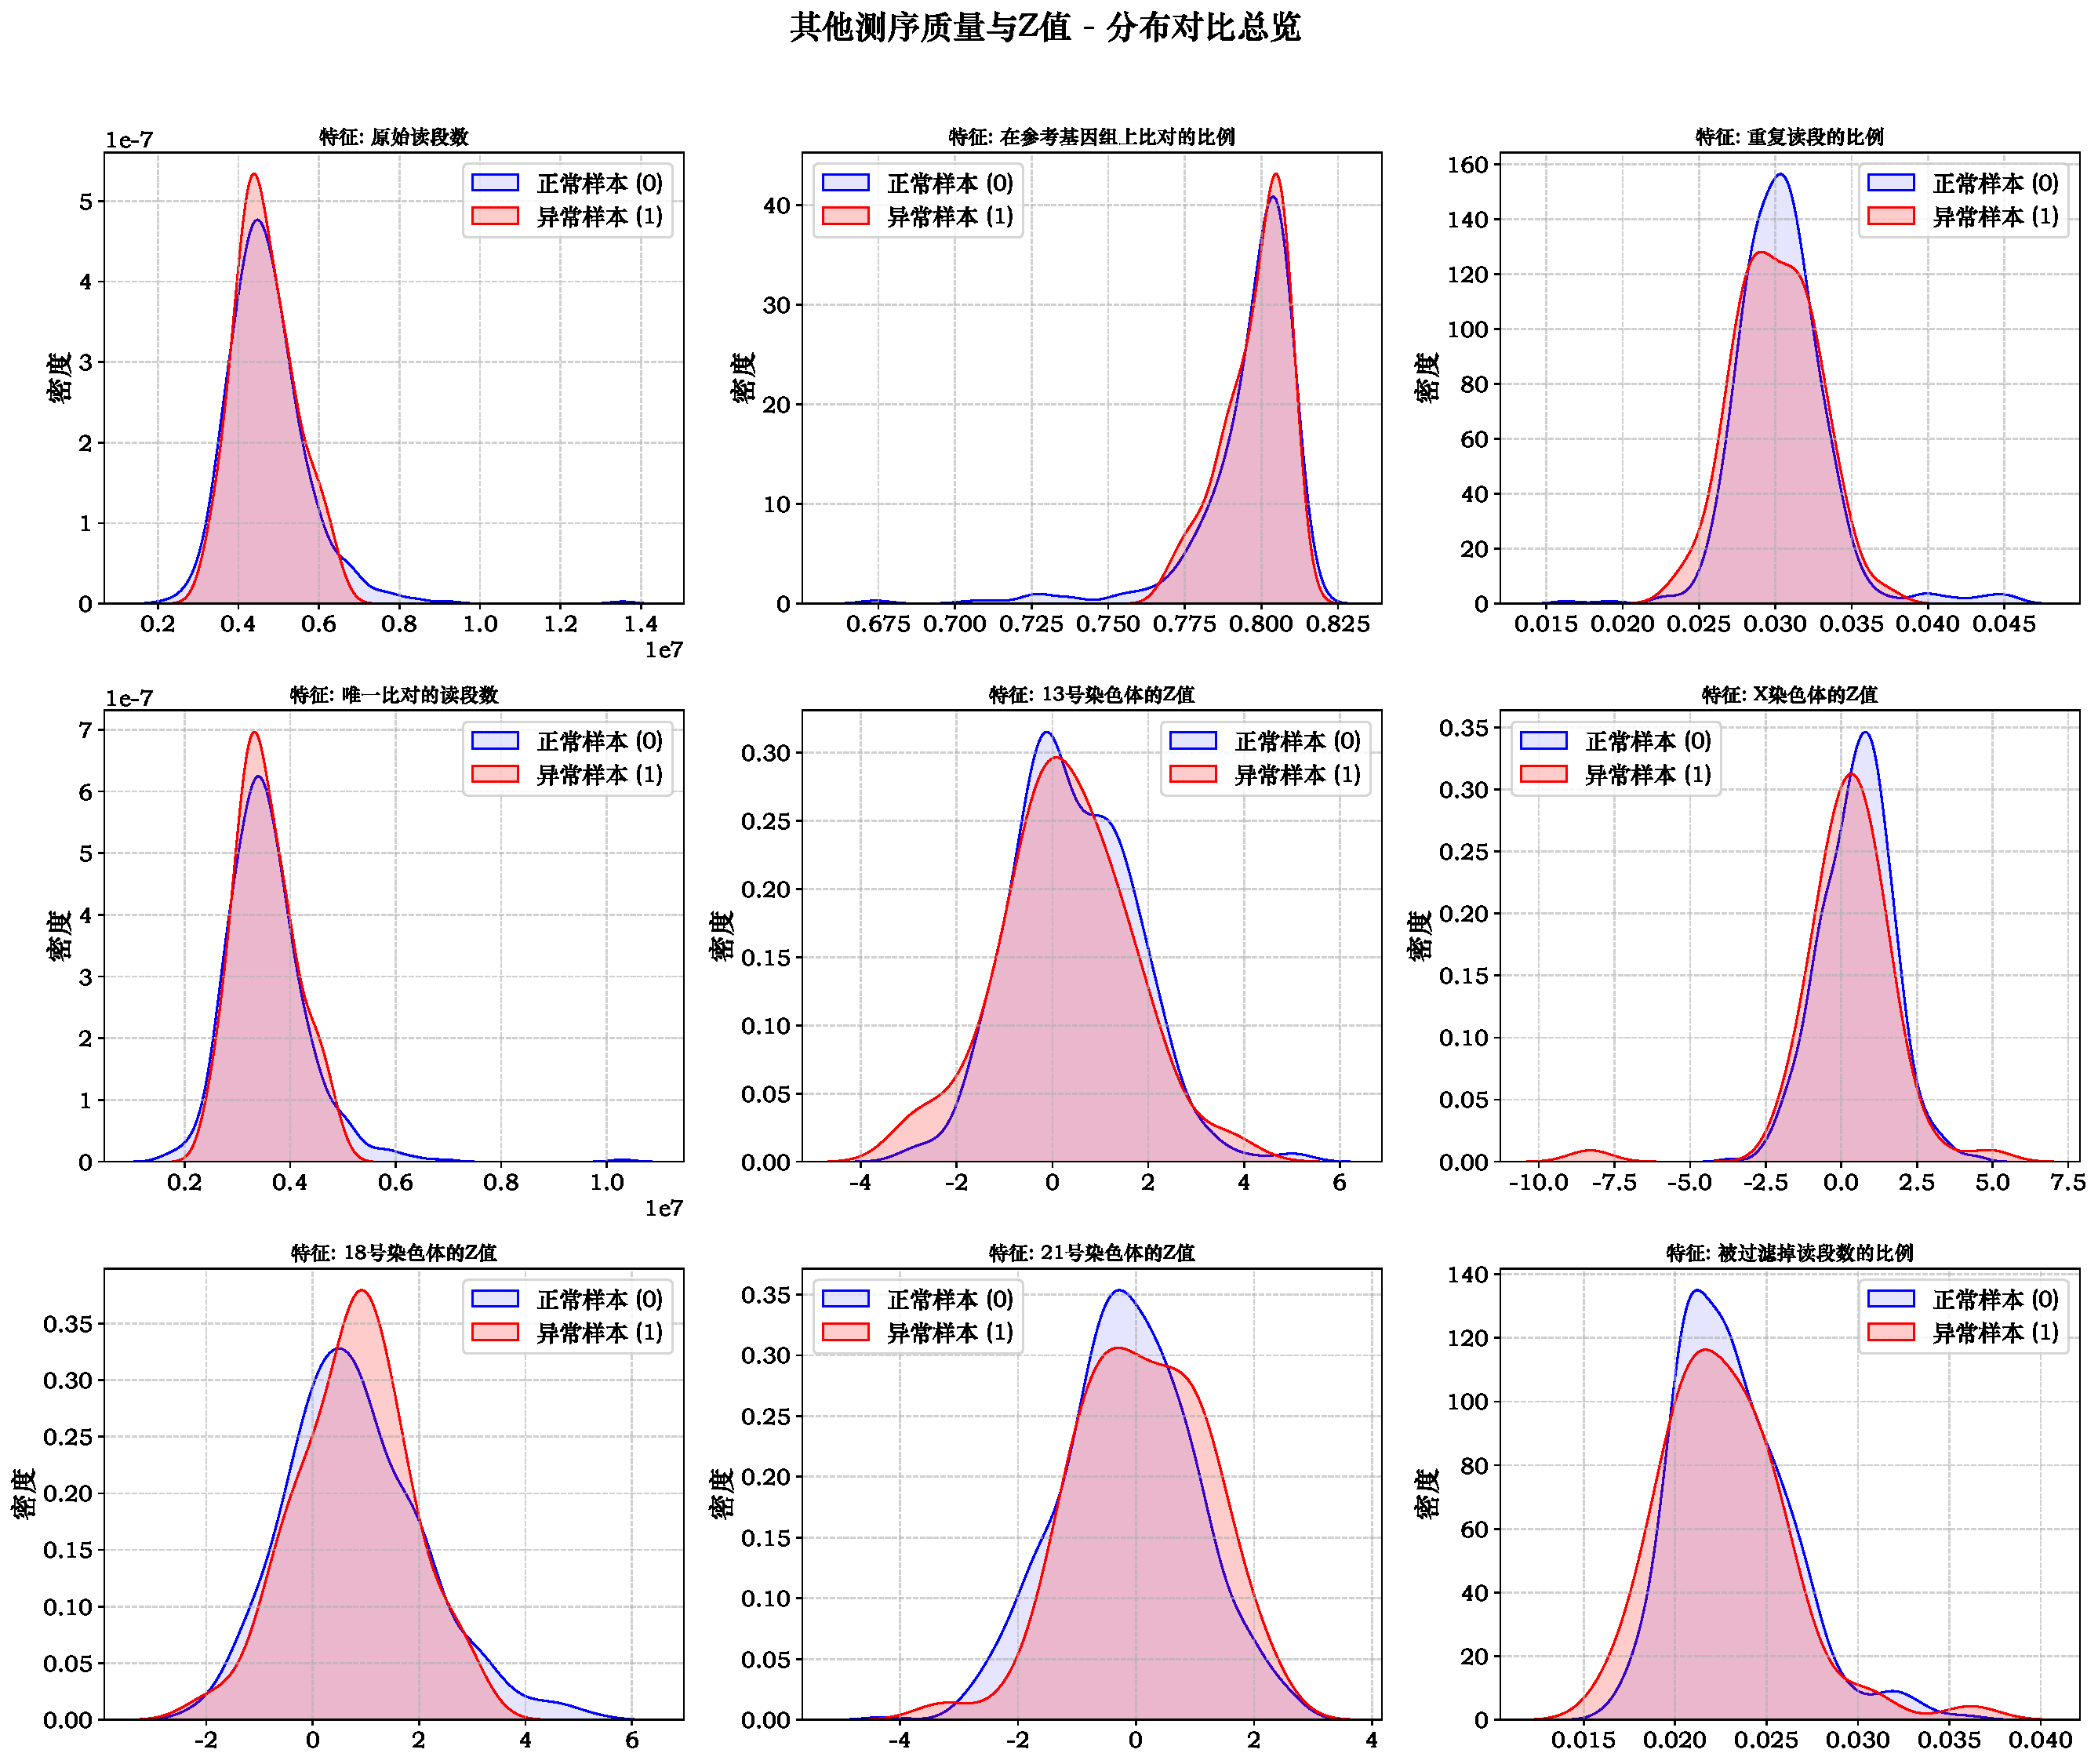
\includegraphics[width=0.9\textwidth]{chapters/Q4/images/其他指标对比图.pdf}
    \caption{其他指标对比图}
    \label{fig:其他指标对比图}
\end{figure}

\addappendix{多重共线性检测}

\lstinputlisting[style=python]{codes/python/Q1/多重共线性检测.py}

\addappendix{非线性混合模型}

\lstinputlisting[style=python]{codes/python/Q1/非线性混合模型.py}

\addappendix{AIC和BIC检验}

\lstinputlisting[style=python]{codes/python/Q1/AIC和BIC检验.py}

\addappendix{KMeans对BMI聚类}

\lstinputlisting[style=python]{codes/python/Q2/KMeans对BMI聚类.py}

\addappendix{加权和法与二周窗口优化}

\lstinputlisting[style=python]{codes/python/Q2/加权和法与二周窗口优化.py}

\addappendix{差分算法}

\lstinputlisting[style=python]{codes/python/Q3/差分算法.py}

\addappendix{GBDT算法}

\lstinputlisting[style=python]{codes/python/Q4/GBDT算法.py}
\end{document}

